\documentclass[answers,11pt]{exam}
\usepackage[utf8]{inputenc}
\usepackage[norsk]{babel}
\usepackage[T1]{fontenc}
% \renewcommand{\rmdefault}{cmss}  % times new roman font
\usepackage{verbatim,a4,amsmath}
\usepackage{epsfig,amssymb,array,delarray}
\usepackage{tabularx,enumerate,alltt,float}
\usepackage{rotating,wrapfig}
\usepackage[font=small,labelfont=bf]{caption}
\usepackage{longtable,color,boxedminipage}
\usepackage{graphicx,lscape,ulem,enumitem,dashbox}
\usepackage[most]{tcolorbox}
\parindent0mm

\usepackage[figurer/]{figurepath}
\usepackage{here,hyperref}

\usepackage{listings}
\usepackage[framed,numbered,autolinebreaks,useliterate]{mcode}
\lstset{inputencoding=ansinew,
literate=  {ø}{{\o}}1%
{æ}{{\ae}}1%
{å}{{\aa}}1%
{Ø}{{\O}}1%
{Æ}{{\AE}}1%
{Å}{{\AA}}1%
}

\textheight210mm
\textwidth145mm
\marginparsep0mm
\oddsidemargin10mm
\parskip 2mm plus 2mm minus 2mm % gir TeX litt fleksibilitet for sidebrekk

\lstset{language=Matlab,
  % basicstyle = \tiny 
}

\begin{document}
\renewcommand{\solutiontitle}{\noindent\textbf{}\par\noindent}
\shadedsolutions
\renewcommand{\thequestion}{\alph{question})}
\renewcommand{\questionlabel}{\thequestion}
\renewcommand{\solutiontitle}{\noindent\textbf{Svar:}\par\noindent}

\renewcommand{\lstlistingname}{Kode}% Listing -> Kode
\renewcommand{\thepage}{\arabic{page}}
\cfoot{\thepage}

\pagestyle{headandfoot}
\runningheadrule
\firstpageheader{}{}{}

\selectlanguage{norsk}
\setlength{\parskip}{0.5cm}

\vspace*{2cm}

\begin{center}
  {\Large \bf ELE130 Anvendt matematikk og fysikk i robotprogrammering}\\[1cm]
  \vspace*{2cm}
  {\LARGE \bf  Øving 2 \\[5mm]
    Introduksjon til \\[2mm]
    simulering i Simulink\footnote{Tilhørende
      filer: \fbox{\tt oving2\_skallfiler.zip} og {\LaTeX}-mal i
      \fbox{\tt oving2\_Overleaf.zip}} }
\end{center}

% ********************************************************
% Fyll inn navnet ditt
% ********************************************************
\begin{tcolorbox}
  {\Large \bf  Levert av John David McGurk}
\end{tcolorbox}

% ********************************************************
% Neste 3 linjer kan kommenteres ut ved innlevering
% ********************************************************
\newpage
\runningheader{Fra {\tt oving2\_intro.tex}}{}{Side \thepage\ av \numpages}
\section*{Om øvingen og innleveringen}

\begin{boxedminipage}{\textwidth}
    \begin{itemize}
      \setlength\itemsep{0mm}
    \item For å bli kjent med Simulink på en effektiv måte,
      er alle oppgavene i denne øvingen svært nyttige, og de vil
      fungere som et oppslagsverk for deg.

  \item For å tilrettelegge for at du skal gjøre flest mulig oppgaver,
    så skal du laste ned og pakke opp \fbox{\tt
      oving2\_skallfiler.zip} som inneholder:
    \begin{itemize}
    \item     Simulink-skallfilen
    \fbox{\tt oving2.slx} hvor deloppgavene a)-p)
    implementeres i egne subsystem
    \item den ferdige modellen \fbox{\tt  oving2\_oppg\_q.slx} for
      deloppgave q)  
  \item skallfilen   \fbox{\tt oving2\_data.m} som
  du må kjøre for 2i),  2o), 2p) og 2q).    
\end{itemize}
    Simulink-skallfilene er spesifisert med trapesmetoden  {\sf ode2 (Heun)} som
    integrasjons\-metode og tidsskritt $T_{s}$ lik 0.01 sekund.

\item  Resultater i scope kan du overføre til en MATLAB-figur med menyvalget
  \dbox{\tt File -->  Print to Figure}, som du igjen kan
     bruke \fbox{\tt LagreMinFigur} på, se prosedyre-boksen nedenfor.
      

    \item   {\color{red}  For å få øvingen godkjent må du gjøre følgende oppgaver:\\
      \fbox{a), c), d),  f), g), i), o), p), q) }}

        \item   Oppgavene 
          \fbox{b), e), h), j), k), l), m), n) } er også lærerike og nyttige, men frivillige.
Dette er markert i toppteksten.       

  \item   {\color{red}  For å ta eksamen i emnet  ELE130 så må denne øving være
  godkjent. Husk at øvingene må leveres individuelt.}


  \item Basis for denne øvingen er
    {\color{blue} kapittel 4  og 5} i  kompendiet. 

    \item På samme måte som i øving 1 finner du en {\LaTeX}-mal i filen 
    \fbox{\tt oving2\_Overleaf.zip}.

  \end{itemize}
  \end{boxedminipage}

 Så langt
det er mulig skal du benytte blokker fra {\sf Eget bibliotek}
  slik at nyttig informasjon om blokkene vises i blokkdiagrammet. Du skal 
  benytte {\sf Scope}-blokkene som heter {\sf Scope, tynne linjer}
  eller {\sf Scope, tykke linjer}  fra {\sf Eget bibliotek} til å
  vise resultatene i.
  Øvingen og skallfilen er organisert  i følgende deler/subsystem:
  \vspace*{-5mm}
  \begin{itemize}
%    \setlength\itemsep{0mm}
  \item ``Om {\sf Integrator}-blokken'', oppgave 2a) - 2e) 
  \item ``Om {\sf Sine Wave}-blokken'', oppgave 2f) - 2h) 
  \item ``Om {\sf Lookup Table}-blokken'',  oppgave 2i) - 2l) 
  \item ``Litt diverse'', oppgave 2m) - 2p)  
  \item ``PID-regulatoren'', oppgave 2q)  
  \end{itemize}


  
I mange av oppgavene skal du inkludere simuleringsresultatet i
innleveringen din og samtidig lese av verdier i MATLAB-figuren.
Prosedyren for å gjøre dette er som følger:
\begin{tcolorbox}[colback=yellow!5!white,colframe=yellow!75!black,
    title=Prosedyre for å lage figur fra
    Simulink-scope og deretter lese av verdier]
       \begin{itemize}
       \item Velg  \dbox{\tt File -->  Print to Figure} fra scopet. Vær
         klar over at eventuelle  avlesningene ved bruk av  {\sf Cursor
           Measurements} ikke blir med i MATLAB-figuren.
       \item Det å avlese/markere i MATLAB-figurer som er laget med utgangspunkt i et
         Simulinkscope gjøres ikke på samme måte som i vanlige
         MATLAB-figurer. Du må nemlig du bruke {\sf Data Cursor}-verktøyet vist i rød ring figuren
         under. For  å avlese mer enn ett punkt, husk å holde inne \dbox{\tt Shift}-knappen.
         \begin{figure}[H]
           \centering
           \scalebox{0.6}{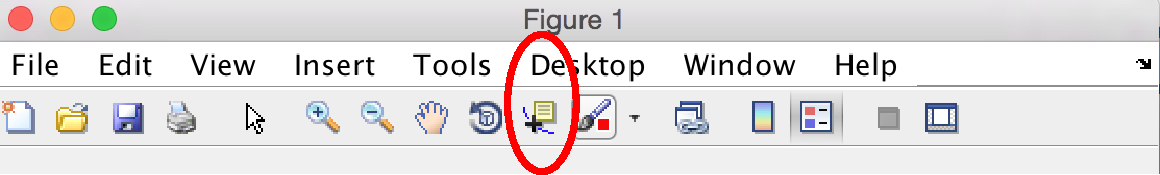
\includegraphics{data_cursor.pdf}}
           \caption{Trykk på knappen i rød ring for å lese av verdier på grafen i en
             figur som er eksportert fra Simulink.  }
         \end{figure}  

       \item Benytt deretter \fbox{\tt LagreMinFigur}-funksjonen til å lage en .pdf av
         figuren. 
       \end{itemize}
       
     \end{tcolorbox}

\label{page:prosedyre}

\newpage

\newpage

\runningheader{Nyttig {\LaTeX}-kode}{}{Side \thepage\ av \numpages}
\begin{tcolorbox}[breakable, enhanced]
  \section*{Forskjellig {\LaTeX}-kode}
  Under er det gitt litt forskjellig kode som du kan kopiere inn i
  svarene under de oppgavene du gjør. Husk bare på å oppdatere
  bokmerkene til nye, unike navn, så slipper du feilreferering.

  \begin{itemize}
    \item    Resultatet fra scopet er vist i figur~\ref{fig:2a}.

          \begin{figure}[H]
            \centering

            \hspace*{0mm}\scalebox{0.35}{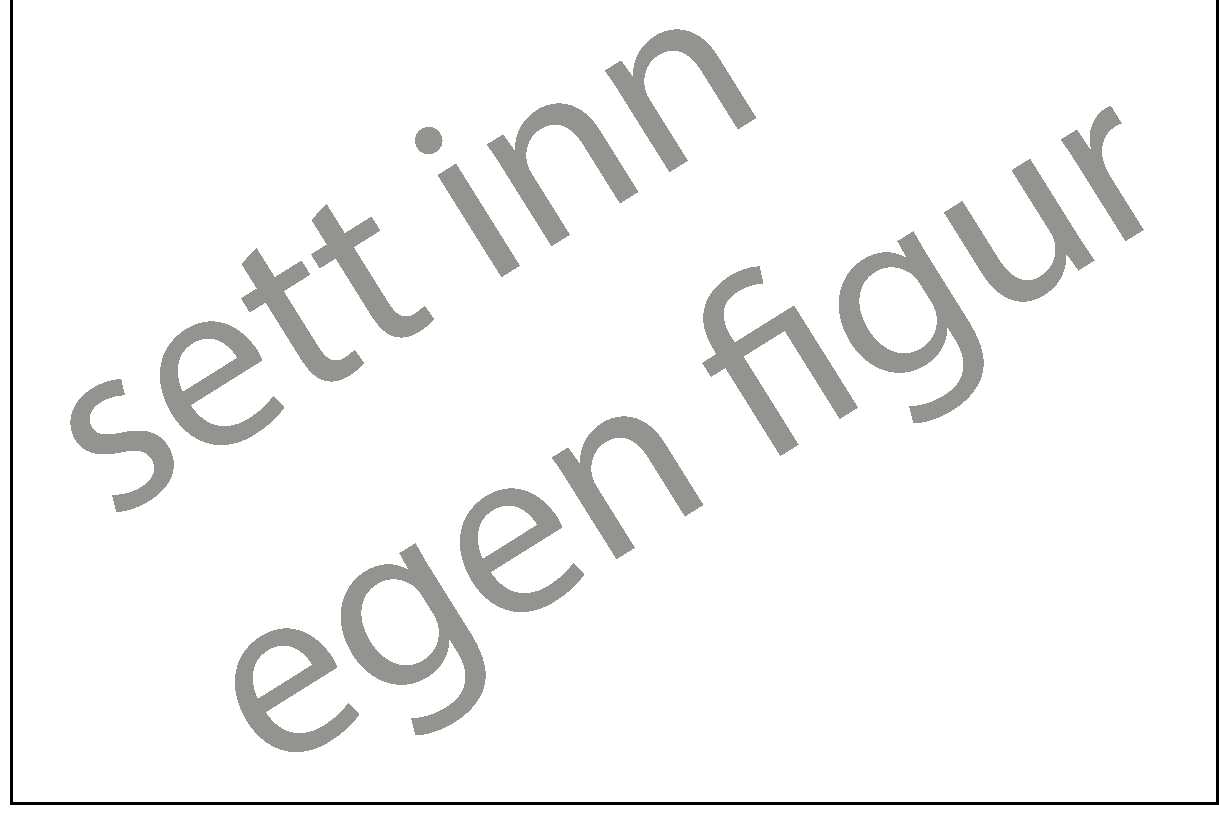
\includegraphics{sett_inn_egen_fig.pdf}}
            \caption{Resultat av blokkskjemaet i modellen. }
            \label{fig:2a}
          \end{figure}

    \item Svaret er gitt i ligning~\eqref{eq:y}.
          For å bruke kommandoen {\tt \textbackslash uuline} må du bruke pakken
            {\tt ulem} som {\tt \textbackslash usepackage\{ulem\}}.
          \begin{equation}
            \label{eq:y}
            y(25) = \uuline{4.2}
          \end{equation}

    \item Eksempel på bruk av {\tt align} er vist i
          ligning~\eqref{eq:integral}.
          \begin{align}
            y(t) & = \int_{0}^{t} U \sin(\omega {\cdot}  \tau) d\tau +
            y(0)\notag                                                 \\
                 & =	 -\frac{U}{\omega}{\cdot}\cos(\omega{\cdot}\tau)
            \Biggl|_{0}^{t}  + y(0)\notag
            \\
                 & =-\frac{U}{\omega}{\cdot}\cos(\omega{\cdot} t)
            -\Bigl(-\frac{U}{\omega}\cos(0)\Bigl) + y(0)\notag
            \\
                 & = -\frac{U}{\omega}{\cdot}\cos(\omega{\cdot}t) +
            \frac{U}{\omega} + y(0)  \label{eq:integral}
          \end{align}

    \item Du finner også mye \LaTeX-kode i hver av .tex-filene til
          delxoppgavene.

  \end{itemize}
\end{tcolorbox}

\newpage
\section*{Om {\sf  Integrator}-blokken}

\begin{enumerate}[label=\alph*)]

  % ********************************************************
  % oppgave a)
  % ********************************************************
  \runningheader{Oppgave a)}{}{Side \thepage\ av \numpages}

\item[]   Alle modellene i denne delen av øvingen skal implementeres
  i subsystemet\\
  \fbox{\tt Om Integrator-blokken, oppgave 2a)-2e)} i 
  skallfilen \fbox{\tt oving2.slx}, og alle modellene skal 
  benytte integratorblokken som numeriske integrerer
  et  inngangssignal $u(t)$ i henhold til
  \begin{equation}
    \label{eq:8}
  y(t) = \int_{0}^{t} u(\tau) d\tau + y(0)
\end{equation}
hvor $y(0)$ er initialverdien.
Vær klar over at alle signalene vi jobber med er
diskrete som $\{u_{k}\}$, men at vi for enkelhets skyld skriver
signalene som kontinuerlige som $u(t)$.



  
% ********************************************************
% oppgave a) 
% ********************************************************
\item


  I denne deloppgaven er $u(t)$ en konstant, og du skal relatere
  simuleringsresultatet til integralregning fra matematikken.
  Implementer modellen vist under.
  \begin{figure}[H]
    \centering
    \hspace*{0mm}\scalebox{0.8}{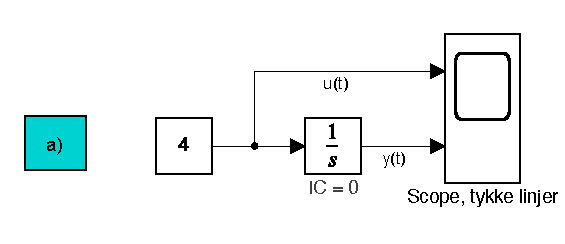
\includegraphics{2a.pdf}}
  \end{figure}
  Utgangen fra {\sf  Constant}-blokken 
  er $u(t)$ og utgangen fra {\sf  Integrator}-blokken
  er  $y(t)$. La  initialverdien til integratorblokken være
  $y(0){=}0$.   {\color{red}La simuleringstiden være 25 sekund.}

  
{\bf Svar på følgende spørsmål:    }
  \begin{enumerate}[label=a\arabic*)]
  \item  Bruk ligning~\eqref{eq:8} og  la $u(t){=}4$. Hva blir det
    matematiske uttrykket for $y(t)$ når $y(0){=}0$?  

  \item  Bruk det matematiske uttrykket til å beregne verdien av $y(t)$ ved
     tidspunkt  $t{=}25$~sekund.
  
   \item Simuler modellen og svar samtidig på følgende spørsmål:
     ``Stemmer simulerings\-resultatet med svaret du fant i  forrige
     delspørsmål?''

     Ta med simulerings\-resultatet i
     innleveringen ved bruke prosedyren på
     side~\pageref{page:prosedyre}.
     
\item  Endre initialverdien til $y(0){=}10$ og simuler. Hvordan endres
  det matematiske uttrykket til $y(t)$? Vis at 
  simuleringsresultatet overstemmer med det matematiske uttrykket. Ta
  med figur i innleveringen.

\end{enumerate}


  \begin{tcolorbox}[breakable, enhanced]
    \subsection*{Svar}

    \begin{enumerate}[label=a\arabic*)]
      \item  Med utgangspunkt i ligning~\eqref{eq:integral}  og
            $u(t){=}4$, er det matematiske uttrykket for $y(t)$ gitt som
            \begin{align}
              y(t) & = \int_{0}^{t} u(\tau) d\tau + y(0) \notag \\
                   & = \int_{0}^{t}4d\tau +0 \notag             \\
                   & = 4 \tau \Big|_0^t \notag                  \\
                   & = 4t - 4 \cdot 0 \notag                    \\
                   & = 4t
            \end{align}

      \item
            \begin{align}
              y(25) & = 4t \notag         \\
                    & = 4 \cdot 25 \notag \\
                    & = 100
            \end{align}

      \item
            Vi ser på grafen at når $x=25$ så er $y=100$, som stemmer med det
            vi fant
            ut i deloppgave a2.
            \begin{figure}[H]
              \centering
              \hspace*{0mm}\scalebox{0.65}
              {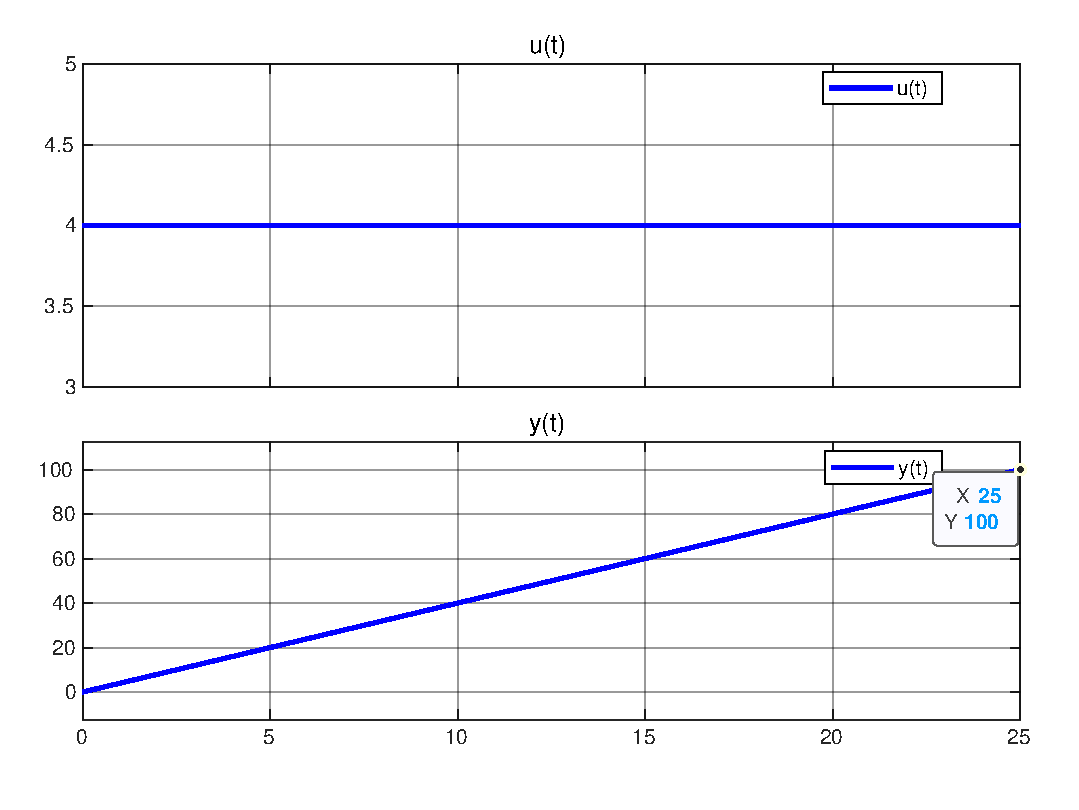
\includegraphics{figurer/a3.pdf}}
              \caption{Resultat av blokkskjemaet i modellen.
                \label{fig:2a1}}
            \end{figure}

      \item
            \begin{align}
              y(t)  & = \int u(t) dt + y(0) \notag \\
                    & = \int 4dt +10 \notag        \\
                    & = 4 t + 10 \notag            \\
              y(25) & = 4 \cdot 25 = 10\notag      \\
                    & = 110
            \end{align}

            Vi ser at dette stemmer med resultatet fra koden i figuren vist
            under.
            \begin{figure}[H]
              \centering
              \hspace*{0mm}\scalebox{0.65}
              {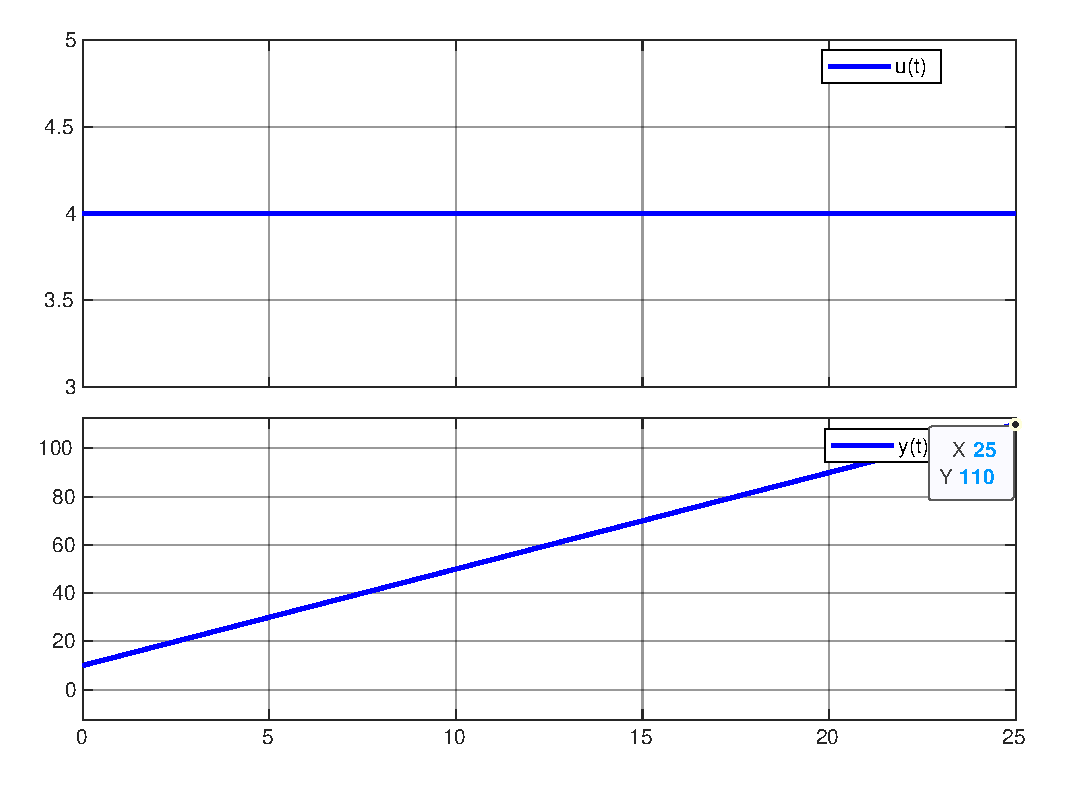
\includegraphics{figurer/a4.pdf}}
              \caption{Resultat av blokkskjemaet i modellen.
                \label{fig:2a2}}
            \end{figure}
    \end{enumerate}

  \end{tcolorbox}

  % ********************************************************
  % oppgave b) 
  % ********************************************************
  \newpage
  \runningheader{Oppgave b), frivillig}{}{Side \thepage\ av \numpages}

% ********************************************************
% oppgave b) 
% ********************************************************  
\item
  Kopier modellen fra a) og bytt ut {\sf Constant}-blokken 
 med en {\sf Step}-blokk som går fra 0 til  4 ved $t{=}5$ som vist
  under
  \begin{figure}[H]
    \centering
    \hspace*{0mm}\scalebox{0.8}{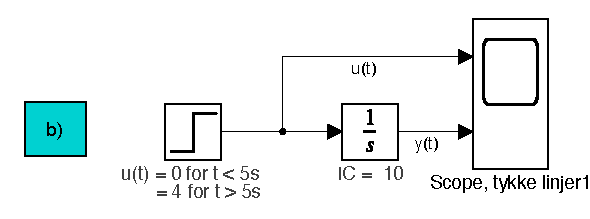
\includegraphics{2b.pdf}}
  \end{figure}
  Uttrykket for $u(t)$ er 
  \begin{equation}
    u(t) =
    \begin{cases}%
      0 & \text{for } t< 5\\
      4  & \text{for } t \geq 5 
    \end{cases}
  \end{equation}
    {\color{red}La simuleringstiden fortsatt være 25 sekund.}

{\bf Svar på følgende spørsmål:    }

  \begin{enumerate}[label=b\arabic*)]
  \item  La initialverdien til integratoren være $y(0){=}10$.
    Simuler modellen og ta med simuleringsresulatet
    i innleveringen din.  Hva er verdien av $y(t)$ i $t{=}25$ sekund?
    Ta med figuren og avlesning
 ved å bruke prosedyren på
     side~\pageref{page:prosedyre}.

   \item Basert på visuell avlesning, hvor stort er arealet under
    $u(t)$? Hvordan henger denne verdien sammen med verdien av $y(t)$?
\item   Endre  $u(t)$ til 
  \begin{equation}
    u(t) =
    \begin{cases}%
      -2 & \text{for } t< 5\\
      2  & \text{for } t \geq 5 
    \end{cases}
  \end{equation}
   Hva blir nå verdien av $y(t)$ i $t{=}25$ sekund?
 Basert på visuell avlesning, hvor stort er nå arealet under $u(t)$?

  \end{enumerate}


  \begin{tcolorbox}[breakable, enhanced]
    \subsection*{Svar (frivilllig)}

    \begin{enumerate}[label=b\arabic*)]
      \item

      \item

      \item

    \end{enumerate}

  \end{tcolorbox}

  % ********************************************************
  % oppgave c) 
  % ********************************************************
  \newpage
  \runningheader{Oppgave c)}{}{Side \thepage\ av \numpages}

% ********************************************************
% oppgave c) 
% ********************************************************  
\item
  Kopier modellen fra a) og bygg den som vist under, hvor initialverdien til integratoren er $y(0){=}0$.
  \begin{figure}[H]
    \centering
    \hspace*{0mm}\scalebox{0.8}{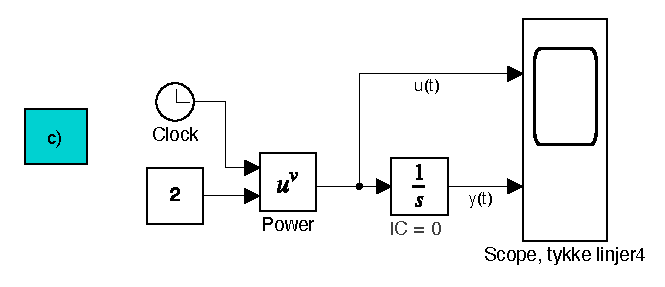
\includegraphics{2c.pdf}}
  \end{figure}
  
  {\color{red}La simuleringstiden fortsatt være 25 sekund.}

    {\bf Svar på følgende spørsmål:    }

  \begin{enumerate}[label=c\arabic*)]
    \item   Hva er det analytiske uttrykket for $u(t)$ som er modellert?
    \item Hva blir det analytiske uttrykket for $y(t)$?
    \item Simuler modell og ta med simuleringsresultatet i
      innleveringen din ved å bruke prosedyren på
     side~\pageref{page:prosedyre}.

\item Vis/forklar at simuleringsresultatet  stemmer
  overens med  det analytiske uttrykket for $y(t)$. 
  
  \end{enumerate}


  \begin{tcolorbox}[breakable, enhanced]
    \subsection*{Svar}

    \begin{enumerate}[label=c\arabic*)]
      \item
            \[u(t) = t^2\]

      \item
            \begin{align}
              y(t) & = \int u(t)dt \notag \\
                   & =\int t^2dt \notag   \\
                   & = \frac{1}{3}t^3
            \end{align}
      \item

            \parbox{\textwidth}{
              \begin{figure}[H]
                \centering
                \hspace*{0mm}\scalebox{0.65}
                {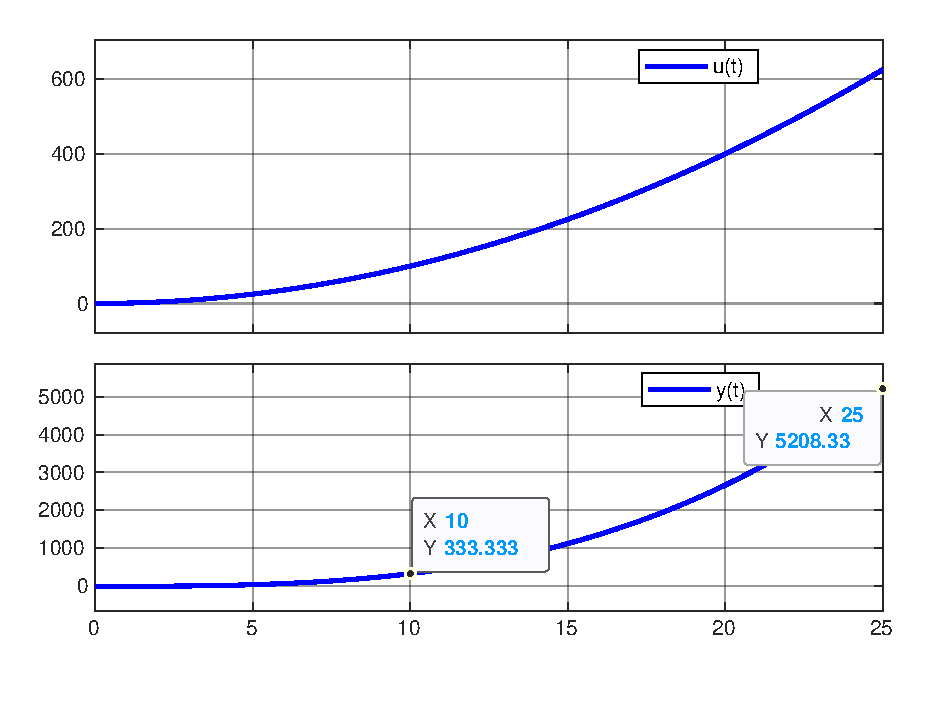
\includegraphics{figurer/c3.pdf}}
                \captionof{figure}{Resultat av blokkskjemaet i
                  modellen.}\label{fig:2c}
              \end{figure}
            }

      \item
            Det er visuelt tidlig at grafen vist i a3 er eksponentielt
            stigende. Vi kan
            sjekke at den stemmer med det analytiske uttrykket ved å sette inn
            $x$ verdiene
            fra grafen inn i utrykket.
            \begin{align}
              y(t)  & = \frac{1}{3}t^3 \notag         \\ \\
              y(10) & = \frac{1}{3} \cdot 10^3 \notag \\
                    & = \frac{1000}{3} \notag         \\
                    & = 333.33 \notag                 \\ \\
              y(25) & = \frac{1}{3} \cdot 25^3 \notag \\
                    & = \frac{15625}{3} \notag        \\
                    & = 5208.33
            \end{align}

    \end{enumerate}
  \end{tcolorbox}

  % ********************************************************
  % oppgave d) 
  % ********************************************************
  \newpage
  \runningheader{Oppgave d)}{}{Side \thepage\ av \numpages}

% ********************************************************
% oppgave d) 
% ********************************************************  
\item
  Lag følgende modell.
  \begin{figure}[H]
    \centering
    \hspace*{0mm}\scalebox{0.8}{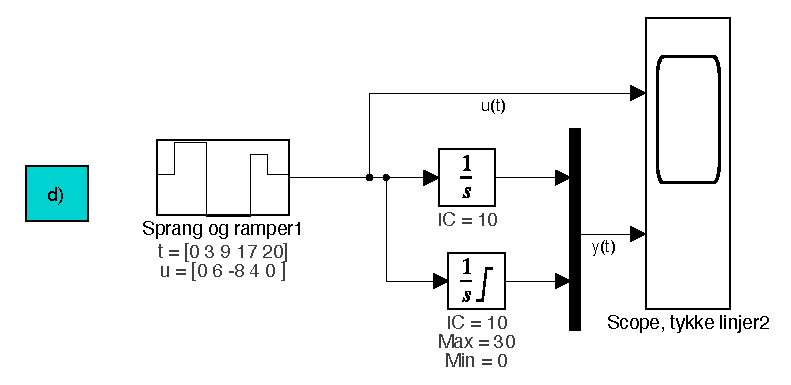
\includegraphics{2d.pdf}}
  \end{figure}
 Signalet $u(t)$ er modellert med {\sf Sprang og
    ramper}-blokken med følgende verdier
  \begin{itemize}
  \item   {\sf Tidspunkter} som {\tt [0~3~9~17~20]}
    \item {\sf Utgangsverdier} som {\tt [0~6~-8~-4~0]} 
  \end{itemize}
  som betyr at
 \begin{equation}
    u(t) =
 \begin{cases}%
  0 & \text{for } 0 \leq t< 3\\
   6  & \text{for } 3 \leq t <9 \\
   -8  &  \text{for }9 \leq t <17 \\
   4  & \text{for } 17 \leq t <20 \\
   0  & \text{for } t \geq 20 
 \end{cases}
  \end{equation}
  Velg interpolasjonsmetode som \dbox{\tt Trappetrinn} fra
    rullegardinmenyen i blokken.  
    Den svarte avlange blokken er en {\sf Mux} som multiplekser flere signal
  inn i samme ``ledning''. Den summerer altså ikke signalene. 
  I blokken {\sf Integrator med begrensing} er
  utgangen begrenset nedad til $y_{min}{=}0$ og oppad til $y_{max}{=}30$. 
   Begge integratorene har  initialverdi $y(0){=}10$. 
  {\color{red}La simuleringstiden fortsatt være 25 sekund.}


  
    {\bf Svar på følgende spørsmål:    }
  
  \begin{enumerate}[label=d\arabic*)]
  \item    Simuler modellen og ta med simuleringsresulatet
    i innleveringen.

\item Forklar med ord hva simuleringsresulatet viser. Forklar først
  den blå kurven, og deretter den røde kurven.

\item Hvordan ville du prinsipielt implementert
      integratorbegrensing i kode?

\item Forklar hva som skjer dersom du prøver å sette initialverdien
  til 40 i \\ {\sf Integrator med begrensing}-blokken?

\item   Hvorfor beholder  $y(t)$ sin verdi når $u(t)$ går
  til 0 fra $t{>}20$~sekund? Hva er den intuitive forklaringen?

\end{enumerate}

  {\color{blue}Vær klar over at du kan skrive både matematiske
    uttrykk,  kommentarer, funksjoner og kode i
  alle feltene i alle Simulink-blokkene. Under vises noen eksempler på hva du kan
  skrive i feltet  {\sf Utgangsverdier}:
  \begin{itemize}
    \setlength\itemsep{0mm}
  \item  {\tt [0~4~0~-5~2]*0.1}
  \item  {\tt [0~-3~2~0~1]  \hspace*{3mm} \%[0~4~0~-5~2] } 
  \item  {\tt randn(1,5)}
  \item  {\tt 1:0.1:1.4}
  \end{itemize}
  Uansett hvilke tall du skriver, så må alltid antall elementer i
  {\sf  Tidspunkter} og {\sf Utgangsverdier} være likt.
}


  \begin{tcolorbox}[breakable, enhanced]
    \subsection*{Svar}

    \begin{enumerate}[label=d\arabic*)]
      \item
            \parbox{\textwidth}{
              \begin{figure}[H]
                \centering
                \hspace{0mm}\scalebox{0.75}
                {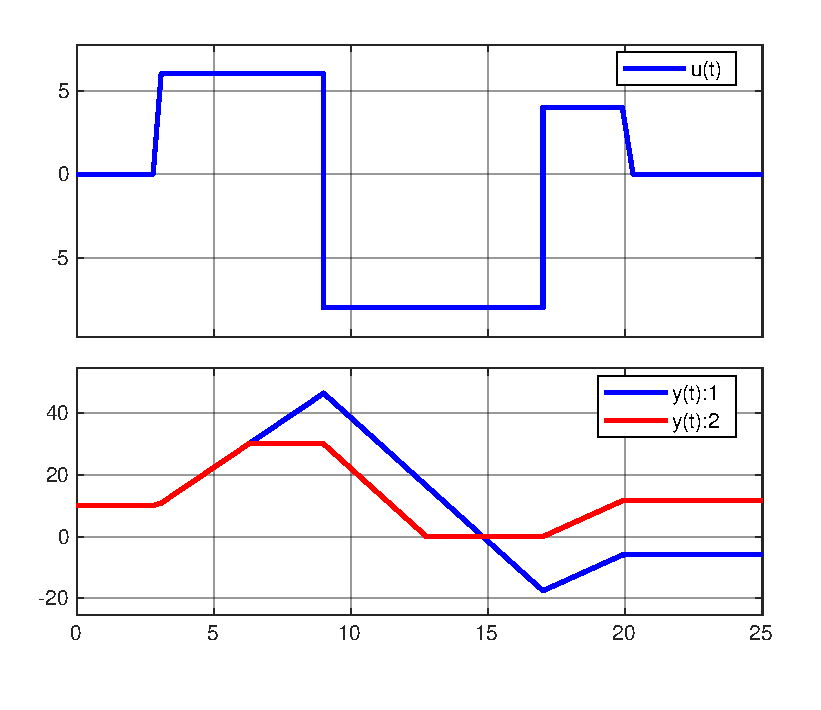
\includegraphics{figurer/2d_svar.pdf}}
                \captionof{figure}{Resultat av blokkskjemaet i
                  modellen.}\label{fig:2d1}
              \end{figure}
            }

      \item
            Den blå kurven viser plottet av den antideriverte/integrerte av
            funksjonen $u(t)$. Den røde viser det samme, men det er satt en
            maks og min grense for funksjonens resultat.

      \item
            Èn måte å implementere integratorbegrensning i kode kunne vaere å
            bruke en if setning for å sjekke om resultatsverdien er over maks
            eller under min, og om så bytt verdien ut hendholdsvis med maks
            eller min verdien.

      \item
            Hvis initialverdien er satt til 40 på integrator med begrensning,
            vil resultatet av $y(t)$ forbli på 0 frem til $u(t)$ går under 0
            (dette skjer
            ved $t=9$ i denne simuleringen). Etter det punktet fortsetter den
            som i tidligere deloppgaver.

      \item
            Den intuitive forklaringen er at $u(t)$ beskriver stigningstallet
            til $y(t)$, altså hvor mye funksjonen stiger eller minker ved en
            gitt
            tidspunkt. Når $u(t)$ går til 0 vil dette si stigningstallet til
            $y(t)$ er 0,
            det vil di den vil verken stige eller minke.
    \end{enumerate}

  \end{tcolorbox}

  % ********************************************************
  % oppgave e) 
  % ********************************************************
  \newpage
  \runningheader{Oppgave e) (frivillig)}{}{Side \thepage\ av \numpages}

% ********************************************************
% oppgave e) 
% ********************************************************  
\item
  Lag følgende modell hvor den nye blokken er {\it  Derivative}. 
  \begin{figure}[H]
    \centering
    \hspace*{0mm}\scalebox{0.78}{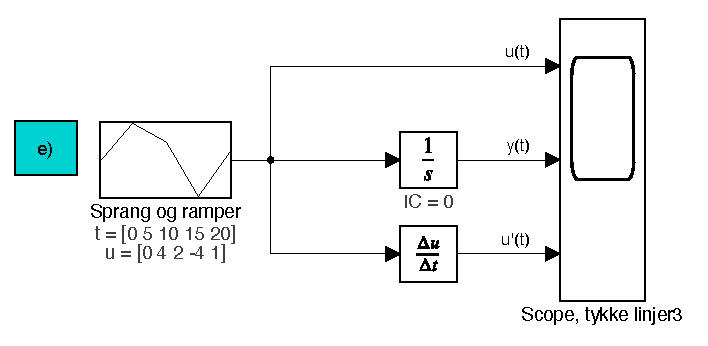
\includegraphics{2e.pdf}}
  \end{figure}
  Signalet $u(t)$ er modellert med {\sf Sprang og ramper}-blokken
  med følgende verdier
  \begin{itemize}
  \item   {\sf Tidspunkter} som {\tt [0~5~10~15~20]}
    \item {\sf Utgangsverdier} som {\tt [0~4~2~-4~1]} 
  \end{itemize}
  og med interpolasjonsmetode som \dbox{\sf Linear} fra
    rullegardinmenyen i blokken.  
  {\color{red}La simuleringstiden fortsatt være 25 sekund.}

    {\bf Gjør følgende oppgaver / svar på følgende spørsmål:    }
  
  \begin{enumerate}[label=e\arabic*)]
    \setlength\itemsep{0mm}
    \item   Simuler modellen og ta med simuleringsresulatet
    i innleveringen din. 
  \item Beregn arealet under $u(t)$ (ta hensyn til både positiv og
    negativt areal).
  \item Hvordan henger dette arealet sammen responsen i $y(t)$?
  \item Hva viser resultatet for den deriverte $u'(t)$? 
    Forklar sammenhengen mellom $u(t)$ og $u'(t)$.
  \end{enumerate}
   


  \begin{tcolorbox}[breakable, enhanced]
    \subsection*{Svar (frivillig)}

    \begin{enumerate}[label=e\arabic*)]
      \item
      \item

      \item

      \item

    \end{enumerate}

  \end{tcolorbox}

  \newpage
  \section*{Om {\sf  Sine Wave}-blokken}

  % ********************************************************
  % oppgave f) 
  % ********************************************************
  \runningheader{Oppgave f)}{}{Side \thepage\ av \numpages}

\item[]   Alle modellene i denne delen av øvingen skal implementeres
  i subsystemet\\
  \fbox{\tt Om Sine Wave-blokken, oppgave 2f)-2h)} i 
  skallfilen \fbox{\tt oving2.slx}.



% ********************************************************
% oppgave f) 
% ********************************************************  
\item
  I denne oppgaven skal du implementere signalet $u(t)$
  \begin{equation}
    \label{eq:208}
    u(t) = 3.2\sin(1.2t)+2
  \end{equation}
  på 2 måter som vist i figuren under. Ved å sammenligne kurvene i
  scopet vil du kunne se at de gir samme resulatet.
  \begin{figure}[H]
    \centering
    \hspace*{0mm}\scalebox{1.2}{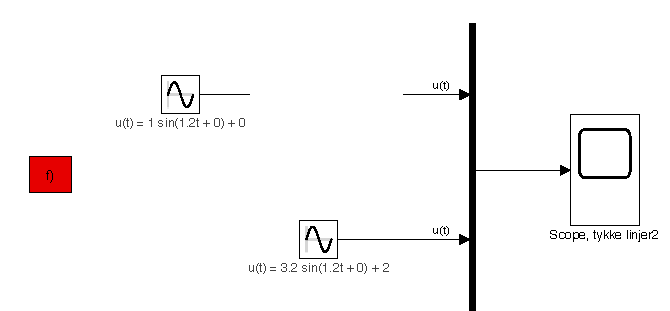
\includegraphics{2f.pdf}}
  \end{figure}

  \begin{itemize}
  \item 
  Den øverste varianten tar utgangspunkt i en 
  {\sf  Sine Wave}-blokk som kun gir ut
  \fbox{$\sin(1.2t)$} med amplitude lik 1 og ingen likevektsverdi (bias).
  Det betyr at du må bygge opp signalet $u(t)$ ved å bruke et utvalg
  av andre blokker, som {\sf  Gain}, {\sf  Constant} og {\sf 
    Sum}. Det er flere måter å gjøre dette på, og detaljene om dette
  er skjult i modellen under. 

\item  Den nederste varianten er  en  {\sf  Sine Wave}-blokk hvor
  amplituden og likevektsverdien til $u(t)$ er spesifisert direkte i blokken.
  \end{itemize}

  {\color{red}La simuleringstiden fortsatt være 25 sekund.  }

      {\bf Gjør følgende oppgaver / svar på følgende spørsmål:    }
  \begin{enumerate}[label=f\arabic*)]
  \item   Bygg ferdig modellen og ta et skjermdump av modellen
    i innlevereringen  din.
    \item  Simuler modellen og ta med simuleringsresulatet
    i innleveringen din.
    For å vise at kurvene ligger over
  hverandre MÅ du endre den  røde kurven til å være  stiplet slik
  at det er mulig  å se at de ligger over hverandre.

  \item   Uttrykket for $u(t)$ i ligning~\eqref{eq:208} kan generelt skrives som
  \begin{equation}
    u(t) = U {\cdot} \sin(\omega{\cdot}t) + u_{A}
  \end{equation}
   Anta at du ikke kjenner til uttrykket for  $u(t)$, men bare har
   kjennskap til figuren med resultatet ditt.
   Vis hvordan du ved hjelp av \underline{kun avlesninger} fra kurven i scopet kan
   beregne estimater av følgende størrelser:
   \begin{itemize}
   \item amplituden  $U$
     \item frekvensen $\omega$ 
   \item likevektsverdien $u_{A}$
   \end{itemize}
   
  \end{enumerate}


  \begin{tcolorbox}[breakable, enhanced]
    \subsection*{Svar}

    \begin{enumerate}[label=f\arabic*)]
      \item
            \parbox{\textwidth}{
              \begin{figure}[H]
                \centering
                \hspace{0mm}\scalebox{0.30}
                {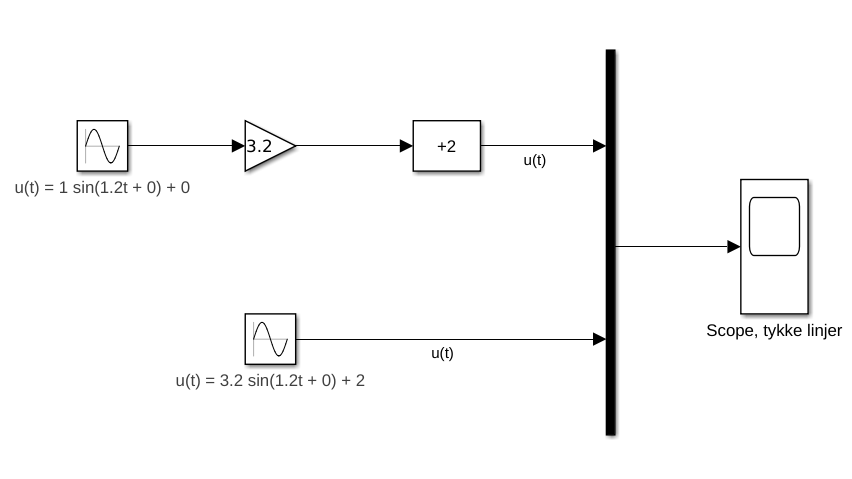
\includegraphics{figurer/2_f1.png}}
                \captionof{figure}{Skjermdump av blokkskjemaet i
                  modellen.}\label{fig:2f1}
              \end{figure}
            }

      \item
            \parbox{\textwidth}{
              \begin{figure}[H]
                \centering
                \hspace{0mm}\scalebox{0.75}
                {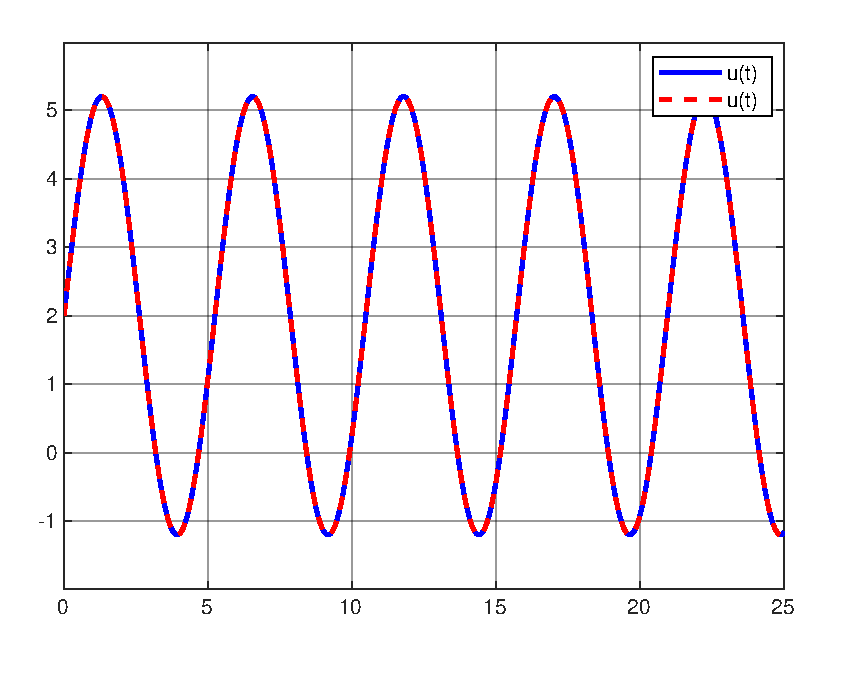
\includegraphics{figurer/2f2.pdf}}
                \captionof{figure}{Resultat av blokkskjemaet i
                  modellen.}\label{fig:2f2}
              \end{figure}
            }
      \item
            Amplituden $U$ kan regnes ut ved å først lese av høy og lavpunkter
            fra grafen og så regne ut $\frac{\text{h{\o}y} + \text{lav}}{2}$.
            Fra denne graven kan vi se høy = 5.2 og lav = 1.2. Setter vi dette
            inn så får vi:
            \begin{align}
              U & = \frac{5.2+1.2}{2} \notag \\
                & =\frac{6.4}{2} \notag      \\
                & =3.2
            \end{align}

            Frekvensen kan regnes ut ved å lese av periodetiden til kurven
            (enklest i dette tilfellet å lese av hvor kurven først går til 0
            med positiv stigning), og så regner vi ut $\frac{2 \pi}{\text{periode}}. Perioden er circa ved 5.24 sekunder her.

    \end{enumerate}

  \end{tcolorbox}

  % ********************************************************
  % oppgave g) 
  % ********************************************************
  \newpage
  \runningheader{Oppgave g)}{}{Side \thepage\ av \numpages}



% ********************************************************
% oppgave g) 
% ********************************************************  
\item
  I denne oppgaven skal du implementere følgende 3 signal ved bruk av  
  en {\sf  Ramp}-blokk og to {\sf  Sine Wave}-blokker.
  \begin{align}
    v_{1}(t) & = 3.2\sin(1.2t)+2 \\
    v_{2}(t) & =
 \begin{cases}%
  1 &\text{for } 0\leq t<15~ \text{sekund}\\
   1+0.3{\cdot}(t-15)   & \text{for } t \geq 15 ~ \text{sekund} 
 \end{cases}\\
    v_{3}(t) & = 1.7\cos(0.7t)+3
  \end{align}
 Legg merke til at $v_{3}$ er et cosinus-signal. 
  Lag deretter et signal $u(t)$ som baserer seg på de 3 signalene på
  følgende måte. 
  \begin{equation}
    \label{eq:208a}
    u(t) = \frac{v_{1}(t)}{v_{2}(t){\cdot}v_{3}(t)} 
  \end{equation}
  Bruk kun én {\sf  Produkt}-blokk til å lage $u(t)$. Send alle 4
  signalene til et scope.
    {\color{red}La simuleringstiden fortsatt være 25 sekund.  }

      {\bf Gjør følgende oppgaver / svar på følgende spørsmål:    }
  \begin{enumerate}[label=g\arabic*)]
\item Bygg modellen og ta med skjermdump av den i innleveringen din.
  \item 
    Simuler modellen og ta med simuleringsresulatet
    i innleveringen din. Vis at du får en figur lik denne.

  \begin{figure}[H]
    \centering
    \hspace*{0mm}\scalebox{0.6}{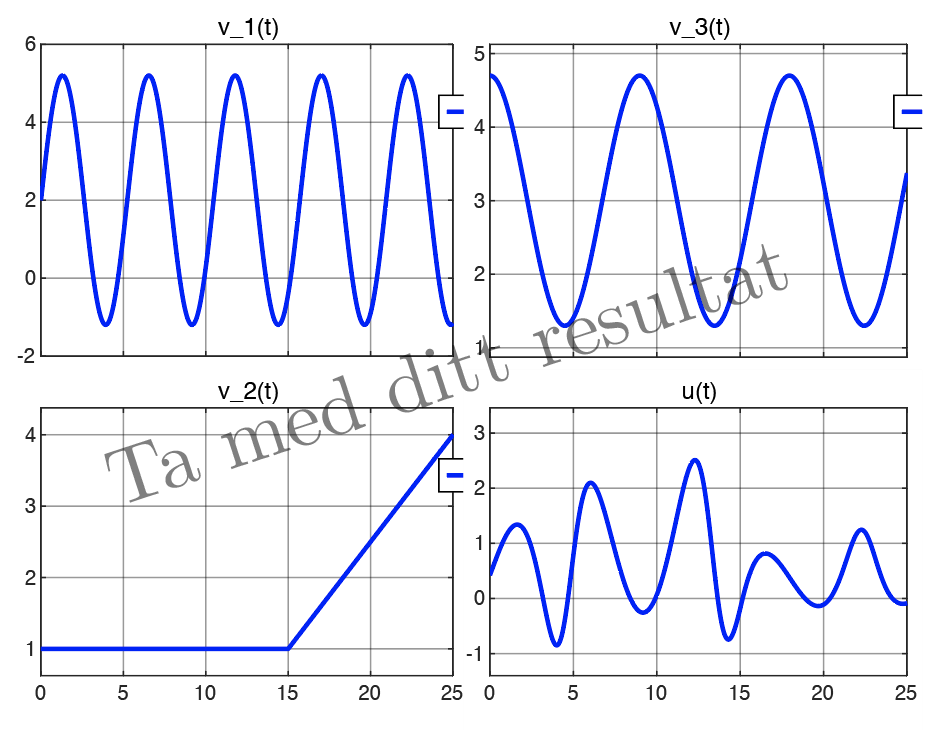
\includegraphics{fig_2g.png}}
    \caption{Simuleringsresultatet}
  \end{figure}

\item Velg et vilkårlig tidspunkt etter $t{=}15$ sekund og les av en verdi
fra $u(t)$. Sett inn samme 
tidspunkt i ligning~\eqref{eq:208a} innsatt $v_{1}(t)$, $v_{2}(t)$ og
$v_{3}(t)$,
og vis at resultatet stemmer med simuleringen. 

    \end{enumerate}


  \begin{tcolorbox}[breakable, enhanced]
    \subsection*{Svar}

    \begin{enumerate}[label=g\arabic*)]

      \item

      \item

      \item

    \end{enumerate}

  \end{tcolorbox}

  % ********************************************************
  % oppgave h) 
  % ********************************************************
  \newpage
  \runningheader{Oppgave h), frivillig}{}{Side \thepage\ av \numpages}

% ********************************************************
% oppgave h) 
% ********************************************************  
\item
  Kopier modellen fra g) og lag et nytt signal som
  \begin{equation}
    \label{eq:209}
    y(t) = 4{\cdot} u(t) {\cdot} t
  \end{equation}
  ved å bruke en {\sf  Gain}-blokk, en {\sf  Clock}-blokk og
  en {\sf  Product}-blokk.

  Utvid {\tt Scopet} til 6 innganger med 6 delfigurer for å vise $v_{1}(t)$,
  $v_{2}(t)$, $v_{3}(t)$,  $u(t)$, $t$ og $y(t)$.
    {\color{red}La simuleringstiden fortsatt være 25 sekund.  }
    Simuler modellen og ta med simuleringsresulatet
    i innleveringen din
    ved å bruke prosedyren på
     side~\pageref{page:prosedyre}.

  \begin{figure}[H]
    \centering
    \hspace*{0mm}\scalebox{0.55}{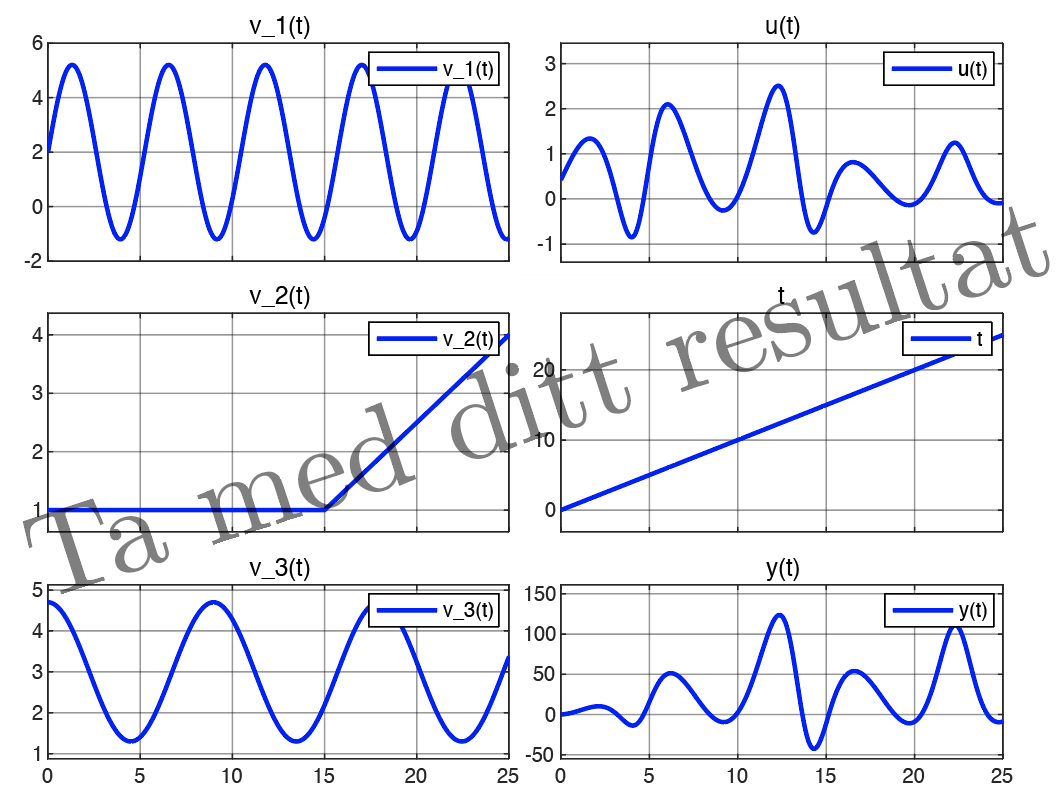
\includegraphics{fig_2h.png}}
    \caption{Simuleringsresultatet}
  \end{figure}



  \begin{tcolorbox}[breakable, enhanced]
    \subsection*{Svar (frivillig)}

  \end{tcolorbox}

  \newpage
  \section*{Om {\sf  Lookup Table}-blokken}

  % ********************************************************
  % oppgave i) 
  % ********************************************************
  \runningheader{Oppgave i)}{}{Side \thepage\ av \numpages}

\item[]   Alle modellene i denne delen av øvingen skal implementeres
  i subsystemet\\
  {\sf  Om Lookup Table-blokken, oppgave 2i)-2l)} i 
  skallfilen \fbox{\tt oving2.slx}.


  % ********************************************************
  % oppgave i) 
  % ********************************************************  
\item
  I denne oppgaven skal du begynne på en ny modell.
  Tettheten til vann som funksjon av temperatur er vist i figuren
  under
  \begin{figure}[H]
    \centering
    \scalebox{0.45}{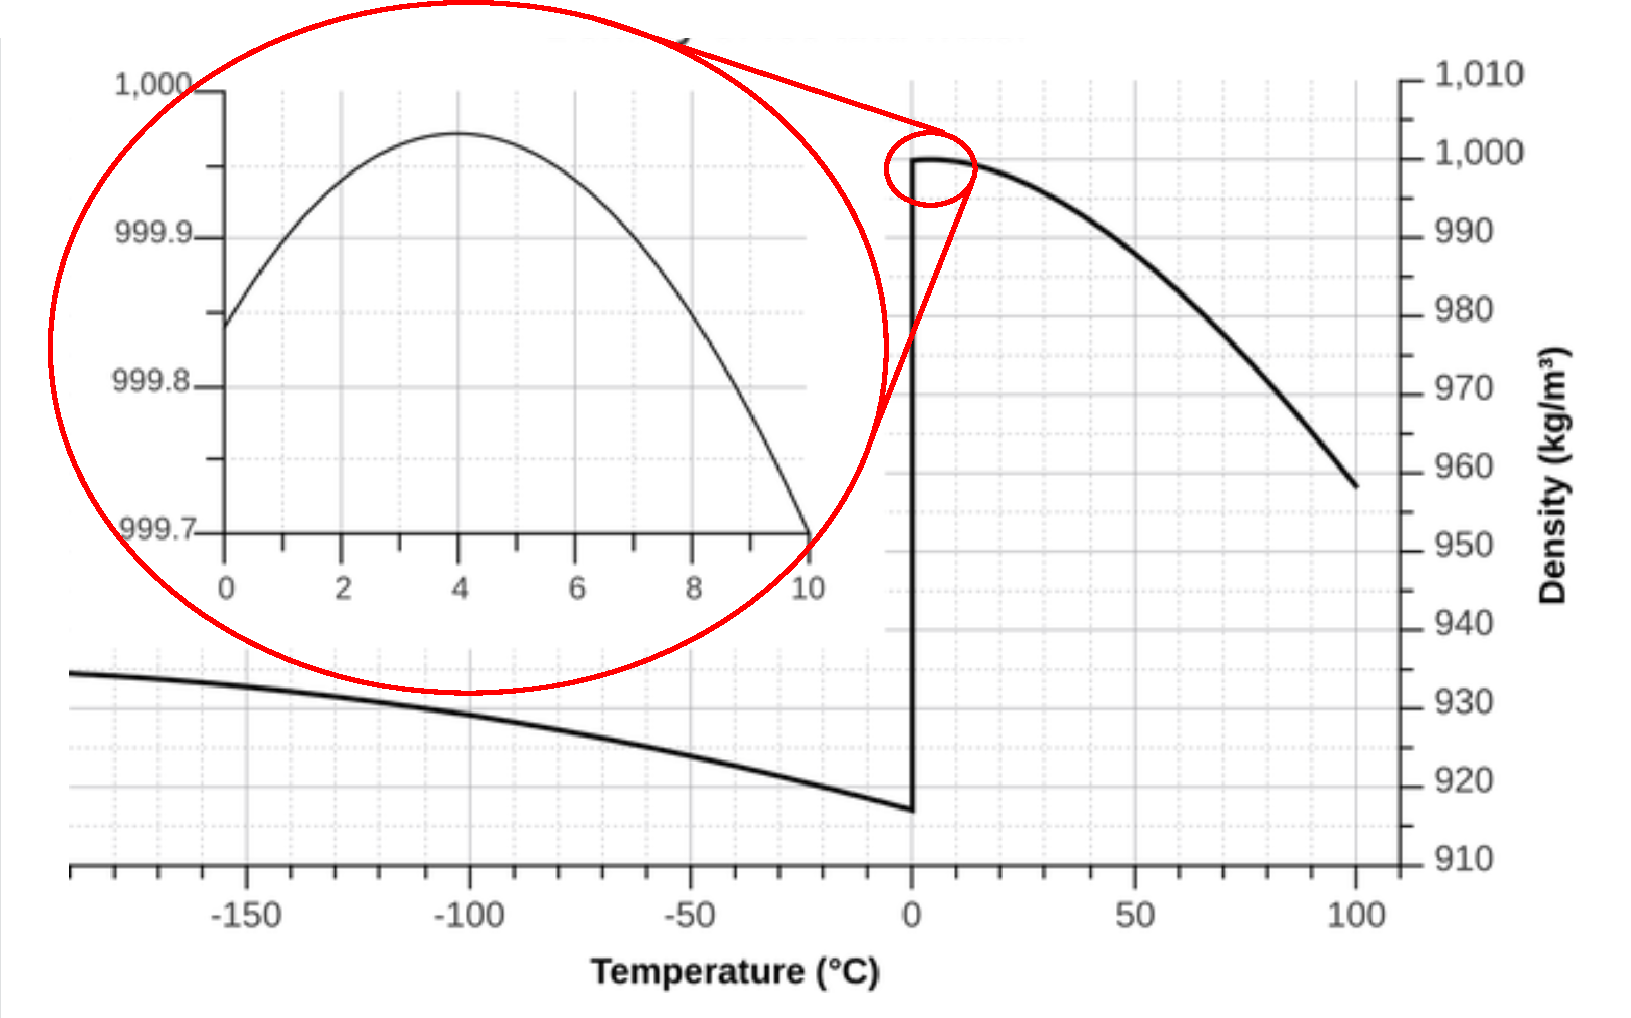
\includegraphics{tetthet_vann.pdf}} 
    \caption{Tettheten vann som funksjon av temperatur. Detaljene mellom
      0 og 10 grader er vist i egen delfigur.}   
    \label{fig:tetthet_vann}
  \end{figure}

  Målet med oppgaven er å implementere sammenhengen i
  figur~\ref{fig:tetthet_vann} i en {\sf  1-D Lookup table}-blokk
  som tar temperatur som et inngangssignal og gir ut tetthet som
  utgangssignal. Denne type blokk brukes for å implementere sammenhenger
  som ikke kan uttrykkes matematisk med en ligning.
  Blokken må spesifiseres med to vektorer med
  tallverdier som representerer kombinasjoner av verdier fra henholdsvis
  x-aksen og
  y-aksen. Ved å interpolere mellom punktene får du en kontinuerlig
  sammenhengen mellom inngangssignalet og 
  utgangssignalet.

  For å få med endringene i tetthet rundt $0^{\circ}$C
  samt detaljene mellom 0 og $10^{\circ}$C vist i  delfiguren i
  figur~\ref{fig:tetthet_vann}, så tar vi 
  utgangspunkt i følgende vektor med 
  temperaturer fra $-150^{\circ}$C til 
  $100^{\circ}$C. Om du vil kan du legge inn flere punkter selv. 

  {\tt T = [-150, -100, -50, -0.001, 0, 2, 4, 6, 8, 10, 30, 50, 70, 100]}

  \begin{itemize}
  \item Åpne skallfilen \fbox{\tt oving2\_data.m} og 
    fullfør den tilhørende vektoren \fbox{\tt rho} med tettheter avlest fra
    figur~\ref{fig:tetthet_vann}. Dette innebærer at for hver verdi i
    vektoren \fbox{\tt T} ovenfor, så leser du av tilhørende tetthet fra
    figuren.

    Ved å kjøre .m-filen får du en figur som viser sammenhengen slik at du
    får bekreftet at du har avlest riktige verdier og riktig antall
    verdier. Hensikten med å bruke en .m-fil først er at det er lettere å
    oppdage feil der enn i selve {\sf Lookup Table}-blokken.   


  \item I Simulinkmodellen henter du inn en {\sf 1-D Lookup table}-blokk
    hvor du benytter disse to
    vektorene til å spesifisere blokken. Du kan nå velge å enten
    kopiere inn vektorene med tallverdier i feltene
    eller skrive \fbox{\tt rho} og \fbox{\tt T} i feltene. Dette
    betinger at du kjører .m-filen først slik av disse variablene er
    tilgjengelig i {\sf Workspace}.

  \item     Måten {\sf 1-D Lookup table}-blokken interpolerer på er bestemt i fanen {\sf  Algorithm}
    under {\sf Interpolation method}. Defaultverdien er som du ser {\sf
      Linear point   slope}.

    
  \item   Fronten på blokken vil vise
    sammenhengen mellom temperatur og tetthet som vist under
    \begin{figure}[H]
      \centering
      \hspace*{0mm}\scalebox{0.8}{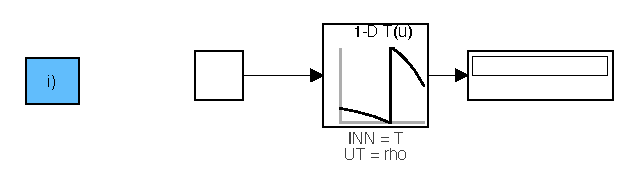
\includegraphics{2i.pdf}}
    \end{figure}

  \end{itemize}

    Inngangen kommer fra en {\sf  Constant}-blokk som representerer 
    temperaturen, og 
    utgangen går til 
    en {\sf  Display}-blokk som viser tilhørende
    tetthet. Du kan dobbelklikke på {\sf Display}-blokken og velge
    \dbox{\sf Numeric  display format} som {\sf Long}.   

    
  {\bf Gjør følgende oppgaver / svar på følgende spørsmål:    }
  
    \begin{enumerate}[label=i\arabic*)]
\item  Skriv inn en av temperaturene fra vektoren {\tt T} og sjekk at
    resultatet gir den verdien du har lest ut fra grafen. Hvilken
    temperatur valgte du, og hvilken tetthetsverdi fikk du ut?

  \item Benytt figur~\ref{fig:tetthet_vann} til å estimere hva tettheten
    er ved $T{=}-20^{\circ}$C. 
    
  \item Verifiser dette ved å skrive inn $-20$ i
    konstantblokka. Hvilken verdi leses av? Ta med 3 desimaler. Husk
    at du må simulere modellen for å lese av.

  \item Skriv inn en svært høy temperatur, f.eks. $T{=}200^{\circ}$C. Hvilken
    tetthet får du da? Hva er det som skjer i blokken siden du får ut et
    tall? Er resultatet fornuftig?

    \item Hvilken tetthet gir $T{=}2000^{\circ}$C? Kommenter gjerne resultatet.
    
  \end{enumerate}



  \newpage

  \begin{tcolorbox}[breakable, enhanced]
    \subsection*{Svar}

    \begin{enumerate}[label=i\arabic*)]

      \item
      \item

      \item
      \item
      \item

    \end{enumerate}

  \end{tcolorbox}

  % ********************************************************
  % oppgave j) 
  % ********************************************************
  \newpage
  \runningheader{Oppgave j), frivillig}{}{Side \thepage\ av \numpages}


% ********************************************************
% oppgave j) 
% ********************************************************  
\item[j)]
  Kopier modellen fra i). Siden temperaturer utenfor
  definisjonsområdet mellom  $-150^{\circ}$C til $100^{\circ}$C gir
  ufysiske tettheter skal du nå begrense verdien på det som
  sendes inn ved å benytte
  en {\sf  Saturation}-blokk som vist under
  \begin{figure}[H]
    \centering
    \hspace*{0mm}\scalebox{0.8}{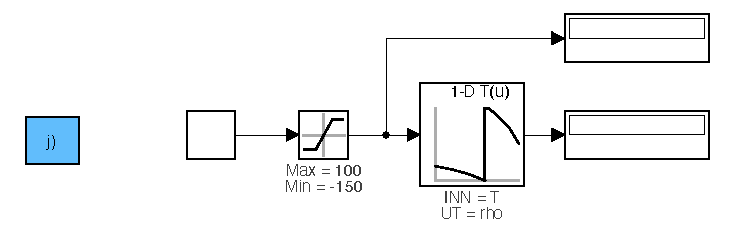
\includegraphics{2j.pdf}}
  \end{figure}
 Spesifiser nedre grense
  lik $-150$ og øvre grense lik 100, og  plasser blokken
  som vist over.

  Legg gjerne til en ny {\sf  Display}-blokk som viser hvilken verdi
  som sendes inn til {\sf 1-D Lookup table}-blokken. 
  
  Test ut med å skrive inn f.eks. $-200$, 200 eller 1000 i {\sf Constant}-blokken.

  {\color{red}La simuleringstiden fortsatt være  25 sekund.}

Ta med skjermdump av
resultatet.


  \begin{tcolorbox}[breakable, enhanced]
    \subsection*{Svar (frivillig)}

  \end{tcolorbox}

  % ********************************************************
  % oppgave k) 
  % ********************************************************
  \newpage
  \runningheader{Oppgave k), frivillig }{}{Side \thepage\ av \numpages}


% ********************************************************
% oppgave k) 
% ********************************************************  
\item[k)]
  Kopier modellen fra j), og erstatt {\sf  Constant}-blokken
  med en {\sf  Ramp}-blokk og bygg modellen om som vist under.

  \begin{figure}[H]
    \centering
    \hspace*{0mm}\scalebox{0.8}{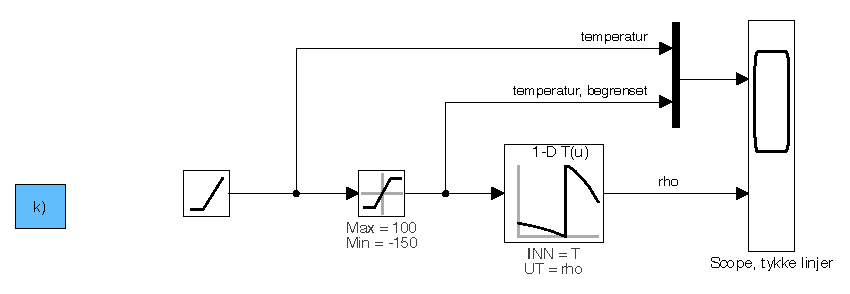
\includegraphics{2k.pdf}}
  \end{figure}

  Spesifiser rampen på en slik måte at
  temperaturen stiger fra $-200^{\circ}$C til $+200^{\circ}$C i løpet av
  simuleringstiden på 25 sekund ut fra følgende sammenheng
    \begin{equation}
    \label{eq:F_tb}
    T(t) = -200 + a{\cdot}t 
  \end{equation}
  {\color{red}La simuleringstiden fortsatt være 25 sekund.  }

      {\bf Svar på følgende spørsmål:    }

\begin{enumerate}[label=k\arabic*)]
        \item Hva blir verdien av $a$?
  \item   Simuler modellen og ta med resultatet i
    innleveringen din.    Forklar hva som skjer i simuleringen.

\item Ved hvilket tidspunktet er temperaturen $T{=}-20^{\circ}$C? Er
  avlest tetthet den samme som i oppgave i)?  
    
\item   Forstørr området mellom $12{<}t{<}17$ sekund på samme måte som
   vist med blå kurve i figur~\ref{fig:akima}.  Få frem at 
  kurven for tettheten består av lineære elementer som viser den lineære
  interpolasjonen som blokken utfører.

  \end{enumerate}
  


  \begin{tcolorbox}[breakable, enhanced]
    \subsection*{Svar (frivillig)}

    \begin{enumerate}[label=k\arabic*)]
      \item

      \item
      \item

      \item

    \end{enumerate}

  \end{tcolorbox}

  % ********************************************************
  % oppgave l) 
  % ********************************************************
  \newpage
  \runningheader{Oppgave l), frivillig}{}{Side \thepage\ av \numpages}


% ********************************************************
% oppgave l) 
% ********************************************************  
\item[l)]
  Kopier modellen fra deloppgave k). For å se forskjellen mellom to aktuelle
  interpolasjonsmetoder, skal du kopiere
  den allerede eksisterende {\sf 1-D Lookup  Table}-blokka og
  legge den i parallell med den første som vist under.
  \begin{figure}[H]
    \centering
    \hspace*{0mm}\scalebox{0.8}{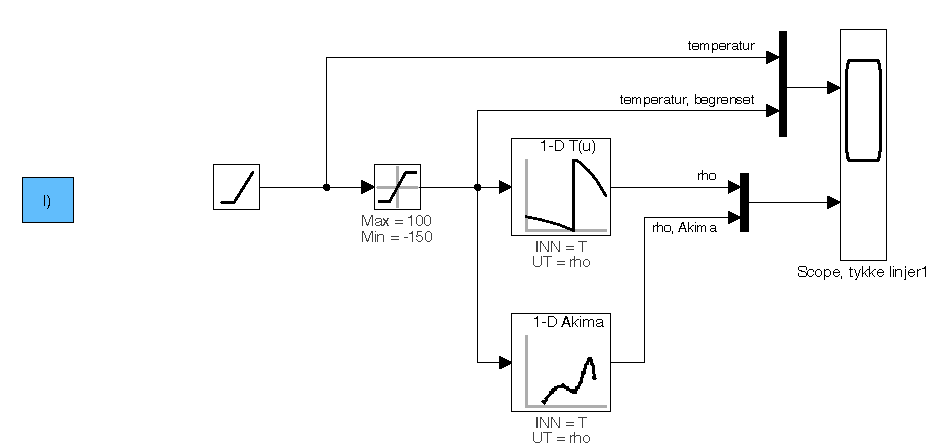
\includegraphics{2l.pdf}}
  \end{figure}
Endre deretter interpolasjonsmetoden i den kopierte blokka
  til  \dbox{\sf Akima   Spline}, sjekk
  {\color{blue}\href{https://en.wikipedia.org/wiki/Akima_spline} 
    {https://en.wikipedia.org/wiki/Akima\_spline}}.
  {\color{red}La simuleringstiden fortsatt være 25 sekund.  }

Simuler modellen på ny, forstørr et område rundt der hvor tettheten er
$\rho{=}1000$, og vis at du får resultatet vist under.
  \begin{figure}[H]
    \centering
    \hspace*{0mm}\scalebox{0.34}{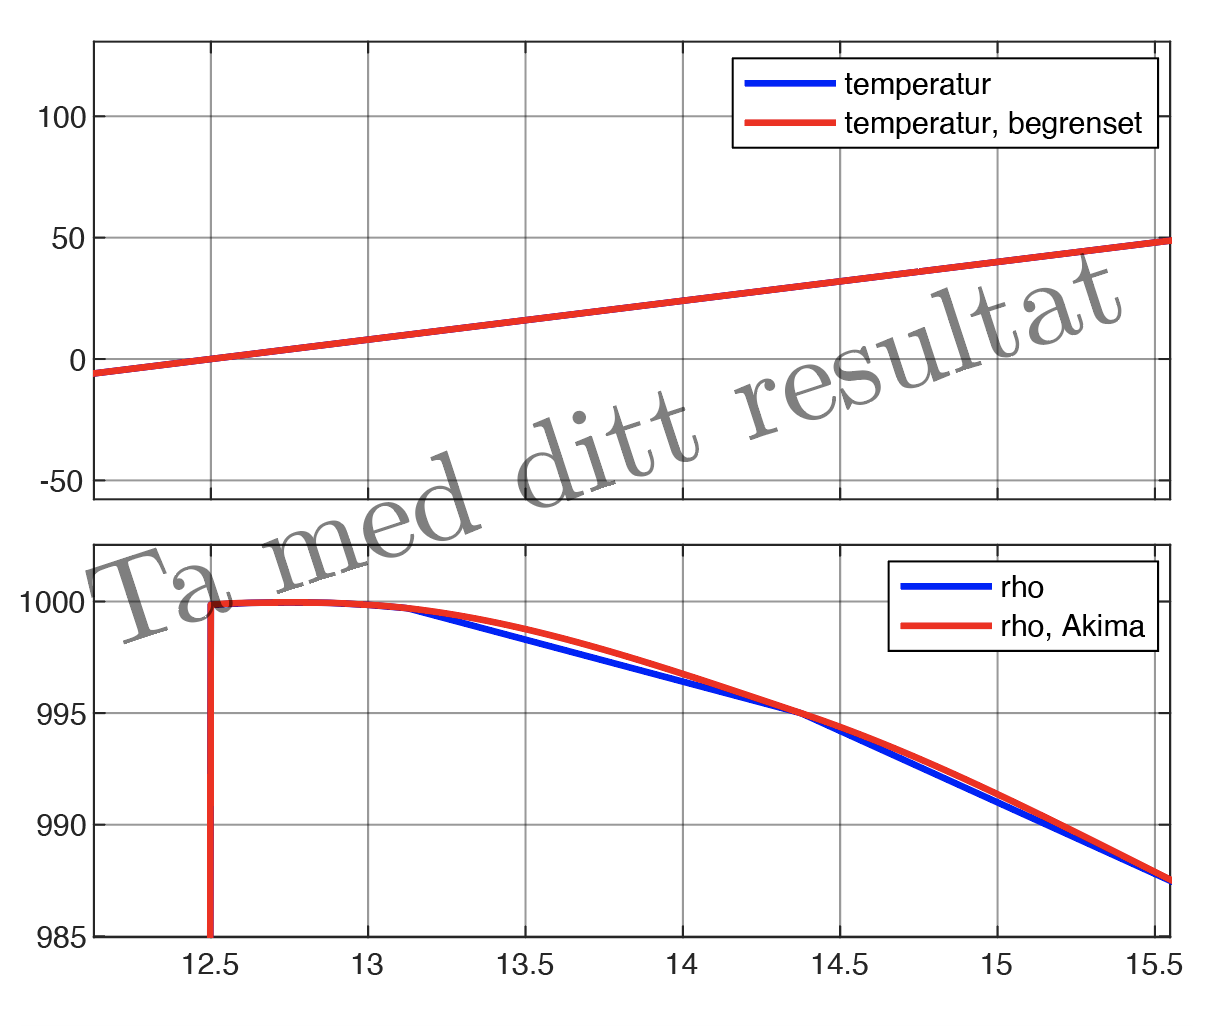
\includegraphics{fig_2l_zoom.png}}
    \caption{Resultat som viser forskjellen på
      interpolasjonsmetodene.}
    \label{fig:akima}
  \end{figure}

  Hva viser resultatet om forskjellen på interpolasjonsmetodene?

  \begin{tcolorbox}[breakable, enhanced]
    \subsection*{Svar (frivillig)}

  \end{tcolorbox}

  \newpage
  \section*{Litt diverse}

  % ********************************************************
  % oppgave m) 
  % ********************************************************
  \runningheader{Oppgave m), frivillig}{}{Side \thepage\ av \numpages}

\item[]   Alle modellene i denne delen av øvingen skal implementeres
  i subsystemet\\
  \fbox{\tt Litt diverse, oppgave 2m)-2p)} i 
  skallfilen \fbox{\tt oving2.slx}.



% ********************************************************
% oppgave m) 
% ********************************************************  
\item[m)]
  Implementer en Simulinkmodell for ligning~\eqref{eq:212}
  \begin{equation}
     a = \sum_{n=1}^{10}n^{2}     \label{eq:212}
   \end{equation}

   Ta utgangspunkt i følgende struktur
     \begin{figure}[H]
    \centering
    \hspace*{0mm}\scalebox{0.8}{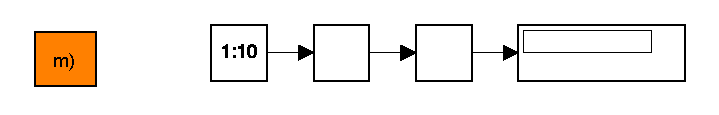
\includegraphics{2m.pdf}}
  \end{figure}
  hvor du ser at i {\sf  Constant}-blokken er 
   tallene for $n$ som \dbox{\sf 1:10} angitt.
   Bruk ellers en {\sf  Math Function}-blokk (velg operasjon fra
   menyen),  en {\sf  Sum of  elements}-blokk og en {\sf 
     Display}-blokk.

   {\color{red}La simuleringstiden fortsatt være  25 sekund.}
Ta med skjermdump av modellen og resultatet.
   


  \begin{tcolorbox}[breakable, enhanced]
    \subsection*{Svar (frivillig)}

  \end{tcolorbox}

  % ********************************************************
  % oppgave n) 
  % ********************************************************
  \newpage
  \runningheader{Oppgave n), frivillig}{}{Side \thepage\ av \numpages}

% ********************************************************
% oppgave n) 
% ********************************************************  
\item[n)]
  Implementer en modell som bruker eksponentialfunksjonen 
   \begin{equation}
     e^{x} 
   \end{equation}
   Ta utgangspunkt i følgende struktur hvor konstantblokken med verdi
   2 innebærer at  $x=2$.

     \begin{figure}[H]
    \centering
    \hspace*{0mm}\scalebox{0.8}{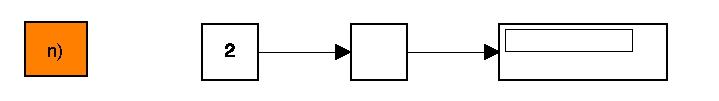
\includegraphics{2n.pdf}}
  \end{figure}
   Bruk igjen 
   en {\sf  Math  Function}-blokk (velg riktig funksjon i menyen)
   og en {\sf    Display}-blokk.

{\color{red}La simuleringstiden fortsatt være  25 sekund.}
Ta med skjermdump av modellen og resultatet.

   


  \begin{tcolorbox}[breakable, enhanced]
    \subsection*{Svar (frivillig)}

  \end{tcolorbox}

  % ********************************************************
  % oppgave o) 
  % ********************************************************
  \newpage
  
\runningheader{Oppgave o)}{}{Side \thepage\ av \numpages}


% ********************************************************
% oppgave o) 
% ********************************************************  
\item[o)]
   Kjør først filen \fbox{\tt oving2\_data.m}, og lag deretter
   modellen vist under
  \begin{figure}[H]
    \centering
    \hspace*{0mm}\scalebox{0.8}{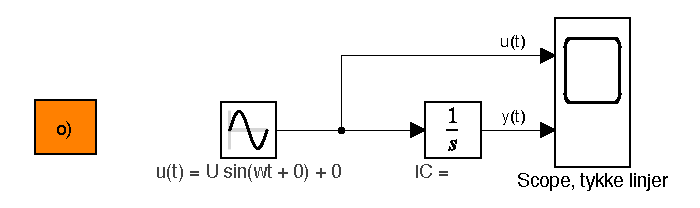
\includegraphics{2o.pdf}}
  \end{figure}
  Som du ser har vi spesifiser $u(t)$ som
  \begin{align}
    \label{eq:1ew}
    u(t) & = U \sin(\omega {\cdot}  t)
  \end{align}
  hvor $U{=}0.5$ og $\omega {=} 0.3$ rad/s gitt i .m-filen.
  Ved å integrere $u(t)$ med initialverdi $y(0){=}0$ finner vi uttrykket
  for $y(t)$ som
  \begin{align}
    y(t)  & = -\frac{U}{\omega}{\cdot}\cos(\omega{\cdot}t) +  \frac{U}{\omega}\label{eq:7aaa}
  \end{align}
  {\color{red}La simuleringstiden nå være 100 sekund, og ikke 25
    sekund som tidligere.  }

  {\bf Gjør følgende oppgaver / svar på følgende spørsmål:    }
  
\begin{enumerate}[label=o\arabic*)]
  \item Sett initialverdien til {\sf 0} i integratoren.
 Simuler modellen og 
    vis at responsen til $y(t)$ alltid er større enn 0. Gi en
    forklaring på hvorfor det er slik.    
    Ta med simuleringsresulatet
    i innleveringen din ved å bruke prosedyren på
     side~\pageref{page:prosedyre}.

  \item   Vi ønsker å få $y(t)$-kurven til å 
  svinge omkring $y{=}0$, og den eneste måten å få dette til på er å
  redusere initialverdien $y(0)$ i integratoren. Bestem ny
  initialverdi som gjør at $y(t)$ svinger omkring $y{=}0$, og simuler på ny.
    Ta med simuleringsresulatet
    i innleveringen din.
  
 

  \end{enumerate}


  \begin{tcolorbox}[breakable, enhanced]
    \subsection*{Svar}

    \begin{enumerate}[label=o\arabic*)]
      \item

      \item

    \end{enumerate}

  \end{tcolorbox}

  % ********************************************************
  % oppgave p) 
  % ********************************************************
  \newpage
  
\runningheader{Oppgave p)}{}{Side \thepage\ av \numpages}


% ********************************************************
% oppgave p) 
% ********************************************************  
  \item[p)]
    I denne oppgaven skal du integrerer
    følgende 3 signal.
\begin{align}
  \label{eq:213}
  u_{1}(t) & = 0.5 \sin(0.3 t) \\
  \label{eq:211}
  u_{2}(t) & = 0.5 \sin(0.55 t)\\
  \label{eq:211s}
  u_{3}(t) & = 0.5 \sin(0.8 t)
\end{align}
Hensikten med oppgaven er å vise hvordan disse 3 sinussignalene henger  
sammen med {\sf Chirp}-blokken. 
Kjør først filen \fbox{\tt oving2\_data.m}, og lag deretter
   modellen vist under
      \begin{figure}[H]
    \centering
    \hspace*{0mm}\scalebox{0.8}{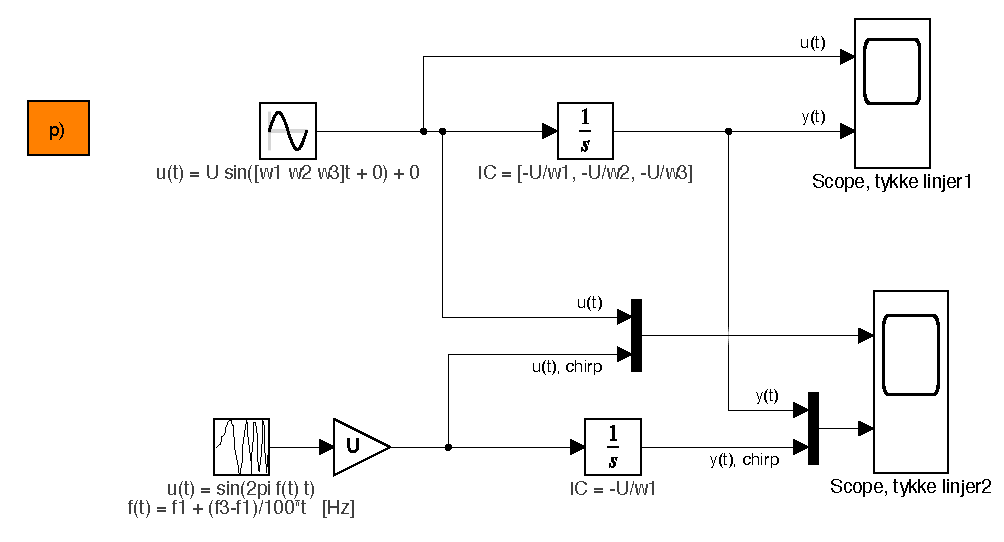
\includegraphics{2p.pdf}}
  \end{figure}
  {\color{red}La simuleringstiden nå være 100 sekund.  }
  
  \begin{itemize}
  \item   I  {\sf  Sine Wave}-blokken
 spesifiserer du {\tt Frequency}-feltet som {\sf [w1, w2, w3]}. 
\item   I  {\sf  Chirp}-blokken
  spesifiserer du
  \begin{itemize}
  \item 
  {\sf f1} som {\tt Initial frequency},
  \item 
  {\sf f3} som {\tt Target frequency} og
  \item 
  {\sf 100} som {\tt  Target time} (tilsvarer simuleringstiden).
  \end{itemize}
  \item Spesifiser initialverdiene som
    vist i figuren slik at cosinuskurvene svinger omkring $y{=}0$.
  \end{itemize}

    {\bf Gjør følgende oppgaver / svar på følgende spørsmål:    }
    
  \begin{enumerate}[label=p\arabic*)]
    \item Simuler modellen og vis at du får et resultat som ligner på 
responsen i figur~\ref{fig:dump_2p}, hvor 
vi har endret den svarte kurven til stiplet slik at
det er lettere å identifisere {\sf Chirp}-signalet.

Ta med simuleringsresulatet
i innleveringen din
ved å bruke prosedyren på
     side~\pageref{page:prosedyre}.

  \begin{figure}[H]
    \centering
    \hspace*{0mm}\scalebox{0.55}{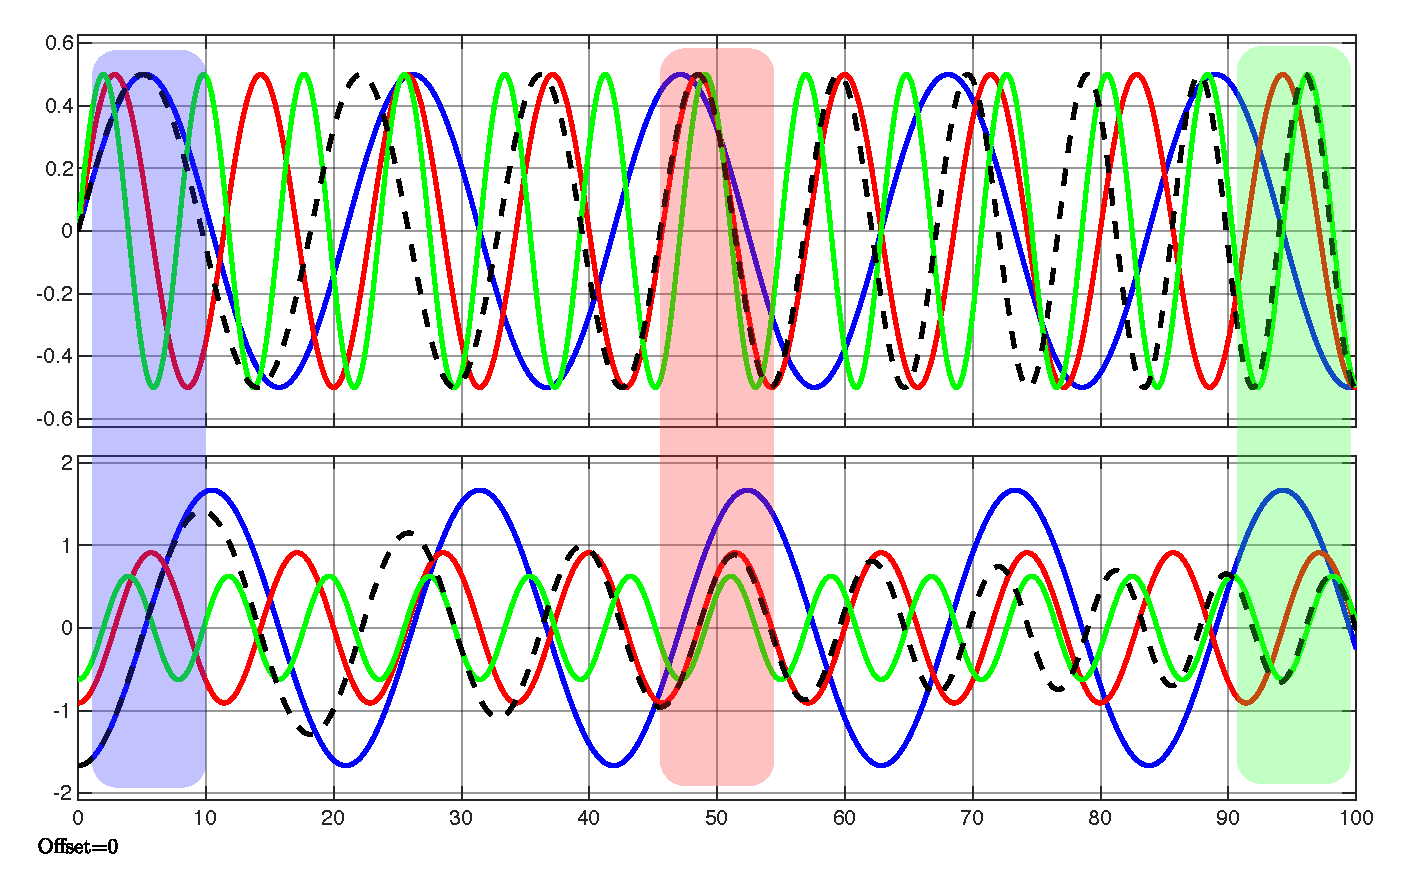
\includegraphics{fig_2p.pdf}}
    \caption{Simuleringsresultat. De fargelagte områdene er gjort i
      tegneprogram etterpå. }
    \label{fig:dump_2p}
  \end{figure}

 Som du ser
``overlapper'' det svart-stiplede chirp-signalet
\begin{itemize}
\item med den blå sinuskurven i det blå feltet i begynnelsen,  
\item med den røde sinuskurven i det røde feltet i midten,  
\item med den grønne sinuslurven i det grønne feltet kurven i slutten  
\end{itemize}
og dette gjelder både i den øverste og nederste delfiguren.


\item Som du ser så reduseres amplituden $Y$ i integralet $y(t)$ når
  frekvensen $\omega$ øker.   
  Forklar, ut fra et matematisk ståsted, hvorfor dette skjer? I
  forklaringen din kan du ta
  utgangspunkt i at uttrykket for $y(t)$ er gitt av
  følgende sammenheng.
\begin{align}
  y(t) & = \int_{0}^{t} u(\tau)  d\tau + y(0)  \notag \\
       & = \int_{0}^{t} U{\cdot}\sin(\omega{\cdot}\tau) d\tau  +y(0) \notag   \\
  & = \ldots \notag   \\
  & = \ldots \notag   
\end{align}

Fortsett på denne utledningen og finn det analytiske uttrykket for
$y(t)$, og bruk dette til å forklare hvorfor amplituden til $y(t)$ synker med
økende frekvens~$\omega$. 
  
\end{enumerate}




 


  \begin{tcolorbox}[breakable, enhanced]
    \subsection*{Svar}

    \begin{enumerate}[label=p\arabic*)]
      \item

      \item

    \end{enumerate}

  \end{tcolorbox}

  \newpage
  \section*{PID-regulatoren}

  % ********************************************************
  % oppgave q) 
  % ********************************************************
  
\runningheader{Oppgave q)}{}{Side \thepage\ av \numpages}


% ********************************************************
% oppgave q) 
% ********************************************************  
  \item[q)]
    I denne oppgaven skal du kun bruke en ferdig modell og ikke
    implementere noe som helst. Hensikten
    er å gi deg litt innsikt i PID-regulatoren som du skal jobbe med i
    det kommende Legoprosjektet.

    PID-regulatoren er den mest brukte regulatoren i industrien, og
    for å forklare virkemåten skal vi benytte en cruisekontroller som
    eksempel og sammenligne med hva som skjer i hjernen vår når vi
    kjører selv, se figur~\ref{fig:neg_feedback3}.
\begin{figure}[H]
  \centering
  \hspace*{5mm}\scalebox{0.38}{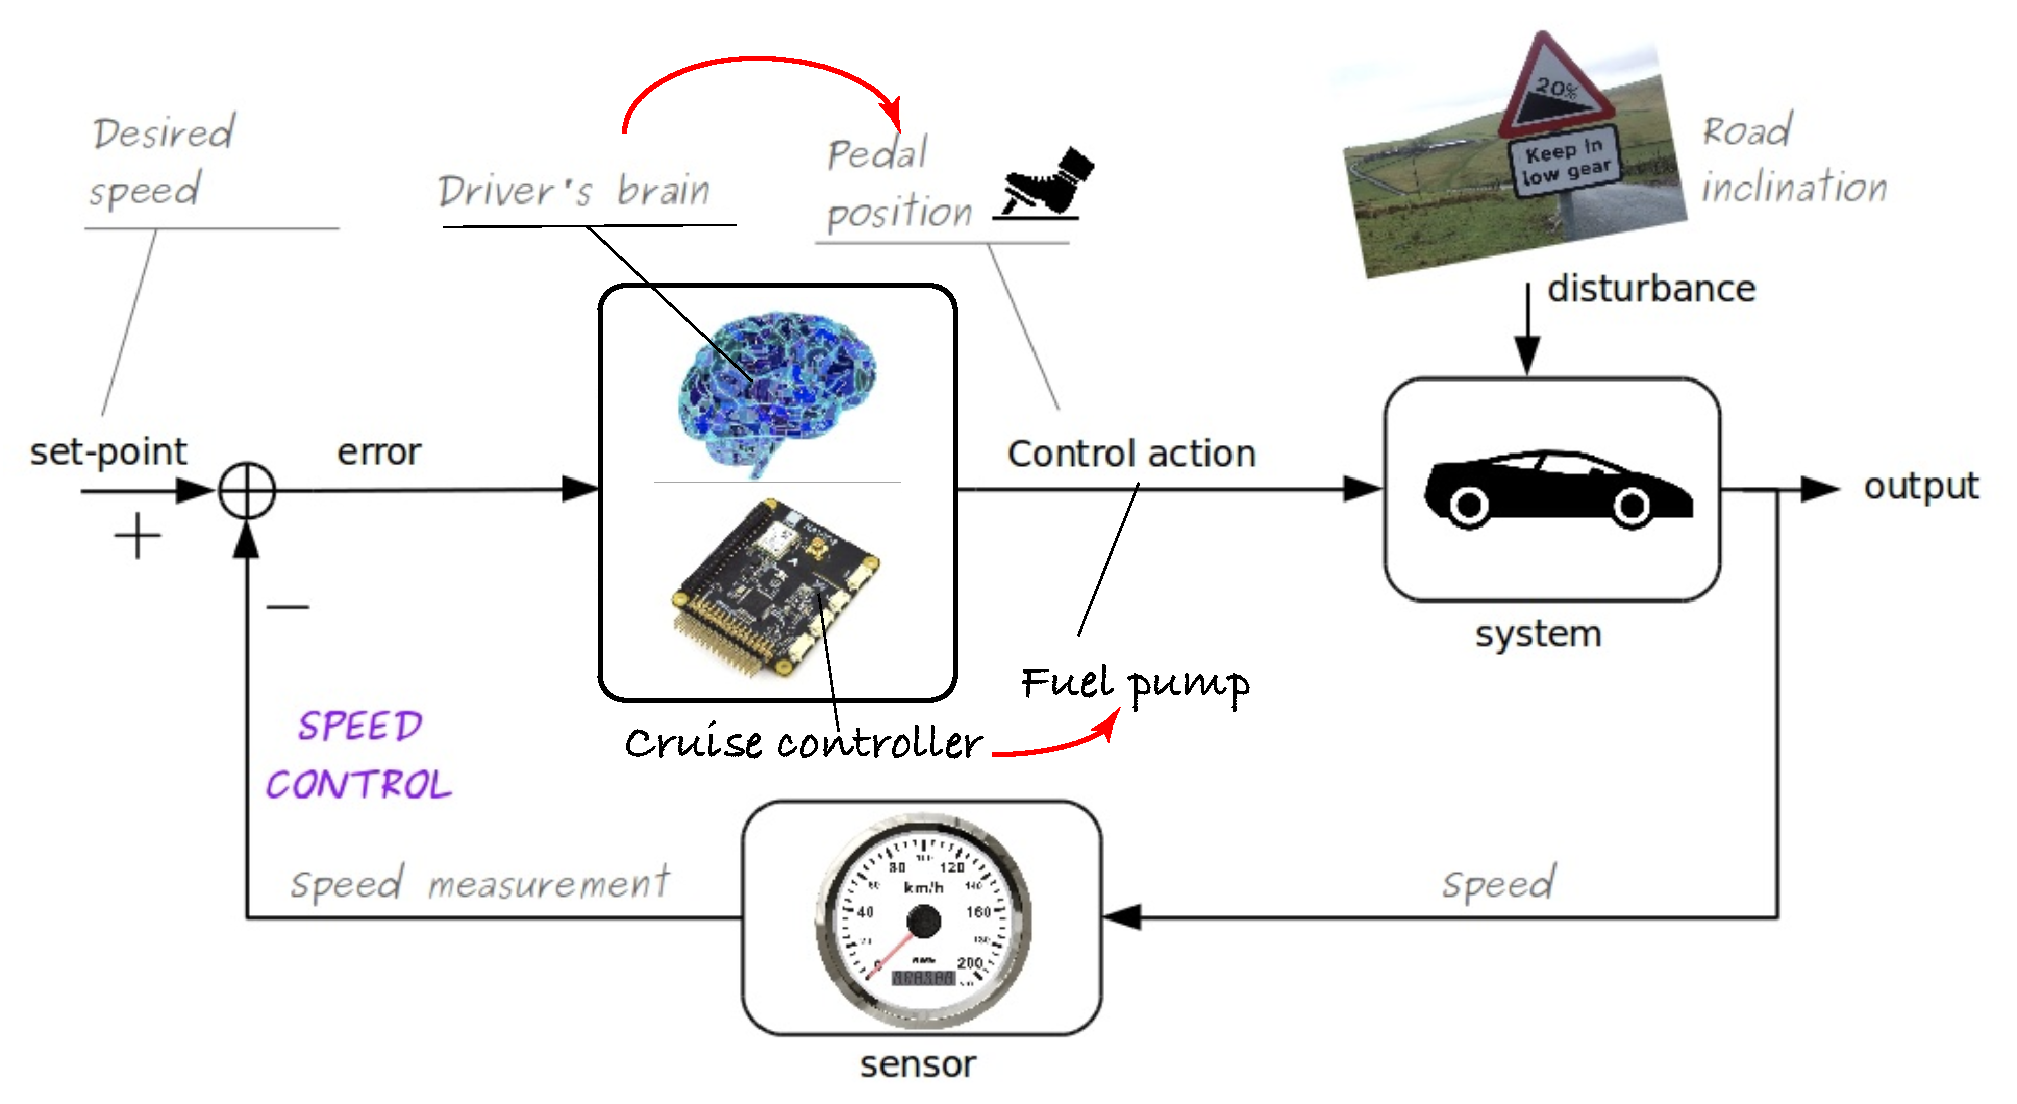
\includegraphics{bil_regulator.pdf}}
  \caption{Prinsippet med negativ tilbakekopling i bilkjøring. Enten
    er det du selv via hjernen din (regulator), øynene dine
    (måleinstrument) og foten din (pådrag) som bestemme farten, eller
    så er det cruisekontrolleren. Hentet fra
    {\color{blue}\href{https://alphaville.github.io/qub/pid-101/}
  {https://alphaville.github.io/qub/pid-101/}}.}
  \label{fig:neg_feedback3}
\end{figure}



Strukturen i figur~\ref{fig:neg_feedback3} kalles
negativ  tilbakekopling, og reguleringssløyfen kan skjematisk
presenteres som i figur~\ref{fig:neg_feedback2}, hvor vi har henviser
til relevante kapitler i kompendiet. 
\begin{figure}[H]
  \centering
  \scalebox{0.55}{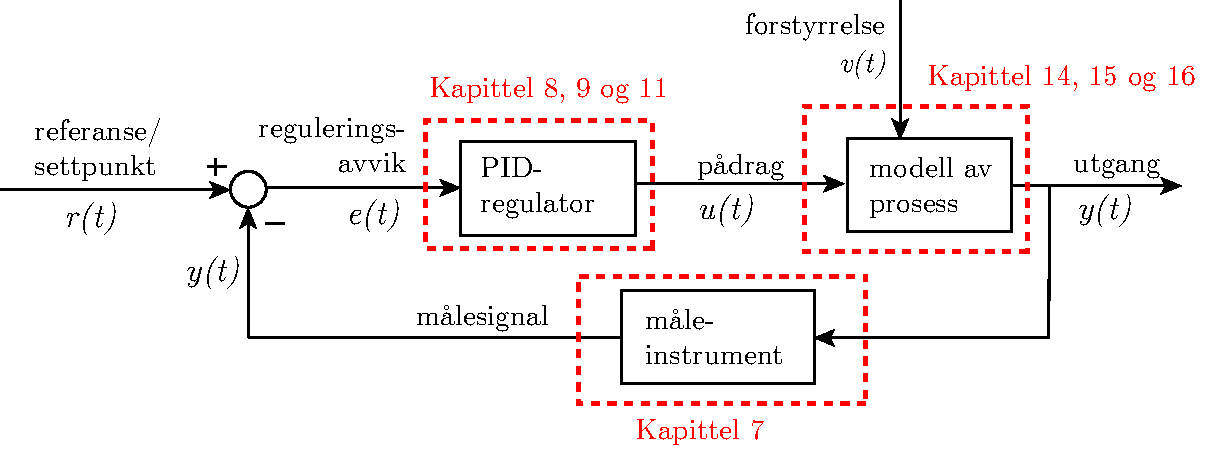
\includegraphics{neg_feedback3.pdf}}
  \caption{Prinsippet for negativ tilbakekopling.}
  \label{fig:neg_feedback2}
\end{figure}
Negativ tilbakekopling innebærer at utgangen $y(t)$ som vi
ønsker å styre/regulere, samples og måles ved hjelp av et
måleinstrument, og dette signalet ``føres tilbake'' og 
sammenlignes med referansen. Siden målingene subtraheres
som markert med minustegnet, oppstår ordet ``negativ''\footnote{Hadde du
  addert $y(t)$ til $r(t)$ ville du 
hatt positiv tilbakekopling.}, og vi 
beregner det såkalte {\it reguleringsavviket} $e(t)$ som
\begin{equation}
  \label{eq:22}
  e(t) = r(t) -y(t)
\end{equation}
Reguleringsavviket er faktisk den eneste informasjonen regulatoren har
tilgang til. {\color{red}Regulatoren har ingen kjennskap til verken
  ønsket verdi $r(t)$ eller utgangens verdi $y(t)$!}
Det betyr at cruisekontrolleren ikke kjenner 
 verken målt fart  eller ønsket fart. Den kjenner kun til 
avviket fra den vilkårlige hastigheten du ønsker å kjøre i.
Poenget er at når avviket $e(t){=}0$, så ``vet'' regulatoren
indirekte at den ukjente målte hastigheten $y(t)$ er lik den ukjente
ønskede hastigheten $r(t)$. En liten kommentar om notasjon:
Strengt tatt er $y(t)$, $r(t)$ og $e(t)$ egentlig diskret verdier gitt
som $\{y_{k}\}$, $\{r_{k}\}$ og $\{e_{k}\}$.


Cruisekontrollen har med andre bare ett mål 
i livet; nemlig å sørge for at $e(t){=}0$ uansett situasjon.
Dette gjelder også
i situasjoner hvor bilen påvirkes av en forstyrrelse~$v(t)$. Tenk på
hva som skjer med hastigheten når du kommer til en
oppoverbakke, som representerer en hindring som reguleringssystemet
ikke har kontroll på. 
Cruisekontrollen oppnår målet i livet sitt ved å beregne et gasspådrag
$u(t)$ som påvirker bilen i en slik retning at målt hastighet $y(t)$
nærmer seg ønsket hastighet $r(t)$, og dermed at $e(t)\rightarrow 0$.
Når du ikke bruker cruisekontroll fungerer du selv som regulator, men
du har jo kontrol på både fart og ønsket fart, men
strengt tatt så gjør du en sammenligning og bruker indirekte avviket
til å enten gi gass eller bremse. 



Matematisk kan PID-regulatoren uttrykkes som ligning~\eqref{eq:10a}, 
hvor ``P'' står for {\it proposjonalvirkning}, ``I'' står
for {\it integralvirkning} og ``D'' står for {\it derivatvirkning}.
\begin{align}
 u(t) = &  \underbrace{K_p{\cdot} e(t)} + 
             \underbrace{\int_0^t K_{i}{\cdot}e(\tau)d\tau} + 
             \underbrace{\frac{d}{dt} \bigr(K_d {\cdot} e(t) \bigl) }   \label{eq:10a}\\
 & \hspace*{13mm} \mathrm{P} \hspace*{18mm} \mathrm{I} 
\hspace*{23mm} \mathrm{D} \notag
\end{align}
hvor $K_p$, $K_{i}$ og $K_{d}$ er forsterkningsfaktorer som kalles
regulatorparametre.
Ligning~\eqref{eq:10a} kan skjematisk
presenteres som figur~\ref{fig:pid_blokk}, hvor P-, I- og
D-delene er representert som tre parallelle bidrag.
\begin{figure}[H]
  \centering
  \hspace*{0mm}\scalebox{0.45}{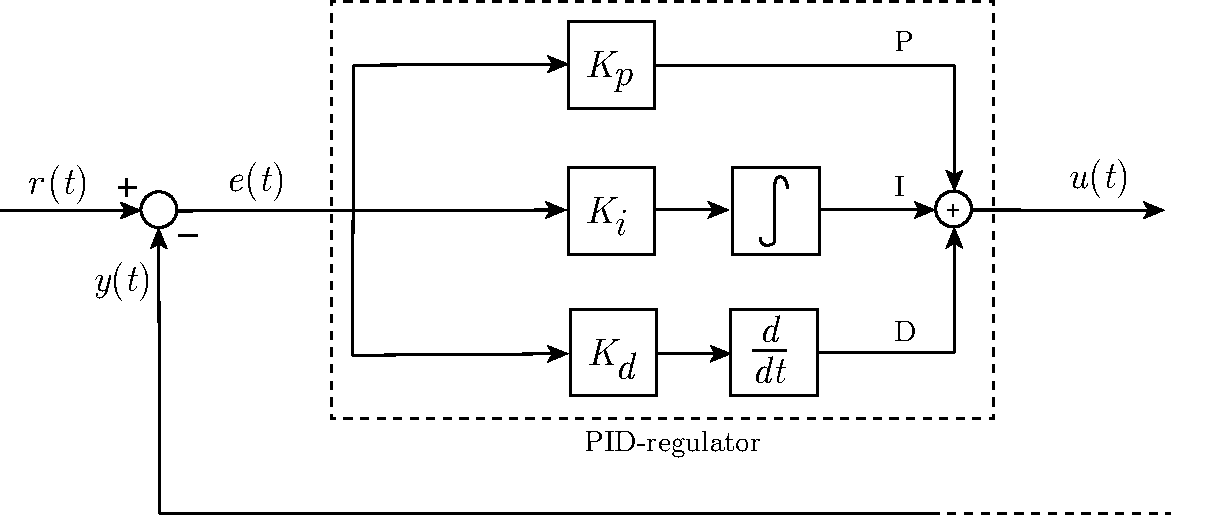
\includegraphics{pid_blokk}}
  \caption{Blokkskjema over  PID-regulatoren i
    ligning~\eqref{eq:10a}.} 
  \label{fig:pid_blokk}
\end{figure}


I simulinkmodellen \fbox{\tt   oving2\_oppg\_q.slx} vist under har 
vi implementert denne PID-strukturen sammen med en
modell av en bil i motbakke.
\begin{figure}[H]
    \centering
    \hspace*{-20mm}\scalebox{0.7}{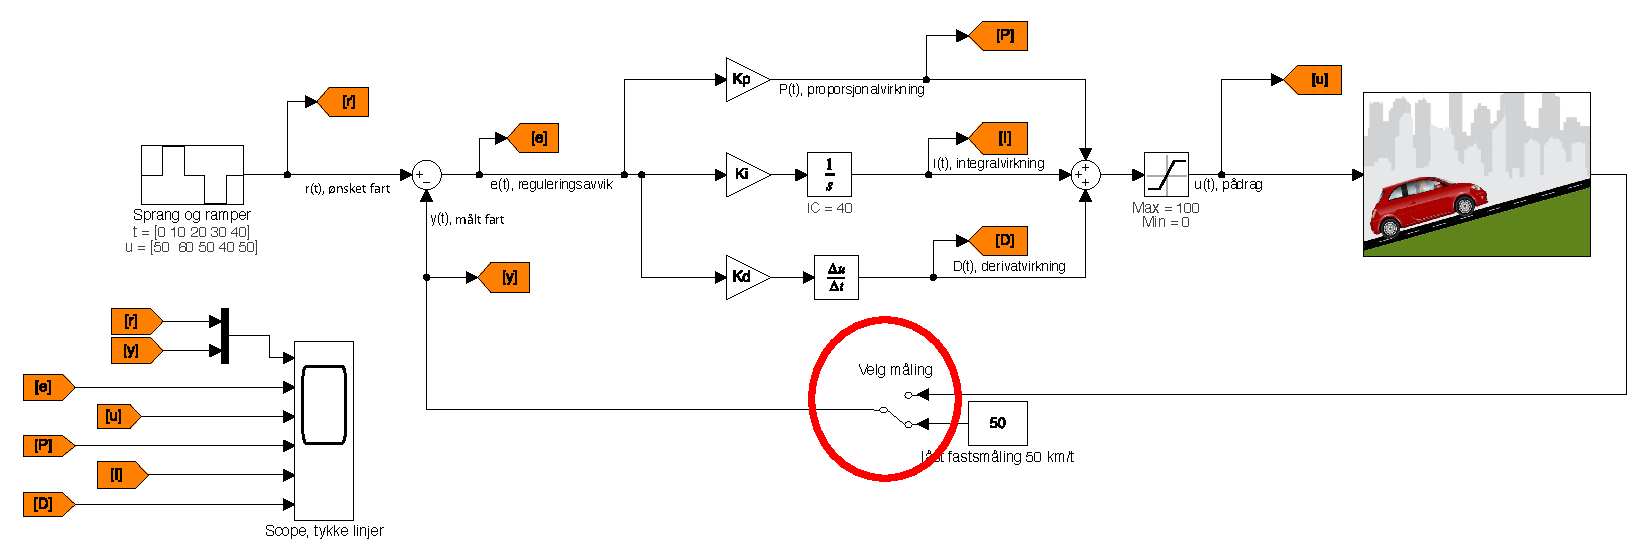
\includegraphics{2q.pdf}}
  \end{figure}
  Situasjonen som er modellert er at bilen kjører i 50~km/t oppover
  en lang bakke, og  pådraget for å oppnå dette er $u(t){=}40$
  (tilsvarer initialverdien til integratoren).
  
Vi har benyttet oss av {\sf  Goto}- og
{\sf   From}-blokker (vist i oransje) slik at modellen blir mindre
spagetti-aktig.  Referansen \fbox{\sf r(t), ønsket fart} helt til venstre
varierer mellom 40 og 60~km/t i løpet av simuleringstiden på 50 sekund.

Den røde ringen markerer en manuell bryter som skifter retning når du
dobbeltklikker på den. Slik bryteren står i figuren antar vi at målt hastighet er
50~km/t uansett hva cruisekontrolleren gjør, og hensikten må å låse
hastigheten er at du skal få anledning til å undersøke hvordan P-, I-,
og D-leddene fungerer før du kopler inn cruisekontrolleren. 

\newpage
    {\bf Gjør følgende oppgaver:    }
    
  \begin{enumerate}[label=q\arabic*)]
  \item  Kjør  filen \fbox{\tt oving2\_data.m}, og simuler modellen og
    bekreft for din egen del at du får responsen i figur~\ref{fig:dump_2q}.
     
  \begin{figure}[H]
    \centering
    \hspace*{10mm}\scalebox{0.7}{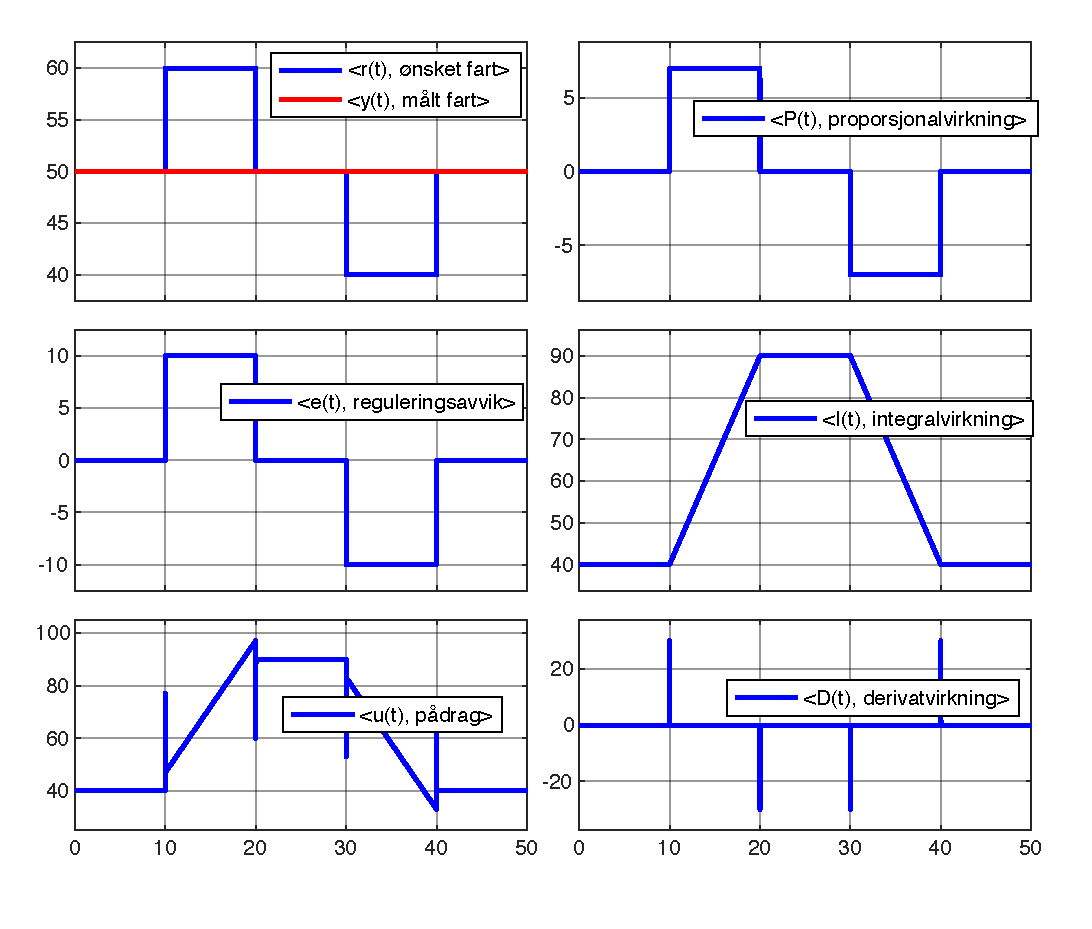
\includegraphics{fig_2q.pdf}}
    \caption{Simuleringsresultat med $K_{p}{=}0.7$, $K_{i}{=}0.5$ og $K_{d}{=}0.03$. }
    \label{fig:dump_2q}
  \end{figure}

  Forklar med dine egne ord hvordan P-, I-, og
  D-leddene fungerer. 

  \item Dobbelklikk på bryteren slik at du måler hastigheten fra
    bilen og at cruisekontrolleren nå er aktiv. Simuler modellen og ta
    med figuren du får i innleveringen. 
    Forklar med ord hva resultatet viser. Fungerer cruisekontrollen
    slik du kjenner den fra din egen erfaring?
  
\item  Endre verdiene av {\sf  Kp}, {\sf  Ki} og
  {\sf  Kd} i m-filen og studere effekten på resultatet. Hvordan
  endres kurvene når regulatorparametrene endres? 
    

 \item Som er frivillig ekstraoppgave kan du prøve å lage din egen
   PID-blokk med din egen meny ved å følge prosedyren i vedlegg~C i kompendiet. 
  
\end{enumerate}




 


  \begin{tcolorbox}[breakable, enhanced]
    \subsection*{Svar}

    \begin{enumerate}[label=q\arabic*)]
      \item

      \item

      \item

      \item

    \end{enumerate}

  \end{tcolorbox}

  \newpage

\end{enumerate}

\end{document}
